\chapter{Methodology}

\section{Optimization \& Genetic algorithms}

As explained in the previous chapter, there are different ways of approaching a multiobjective optimization problem. Three different ways will be analyzed in order to choose the most appropriate one for the coupling of a search method and computer fluid dynamics: 

\begin{itemize}
    \item Random search: this method is also known as Monte Carlo method. It consists of sampling the search space in a random fashion and hoping to get a good definition of the Pareto front. As said before this kind of methods are not very efficient and in order to achieve high accuracy values, the number of individuals must be big enough. Furthermore, this approach is only efficient in 2 and 3 variable search spaces, given that with more than 3 variables, the search space is too big to cover it with a simple sampling of points.
    \begin{figure}[h!]
        \centering
        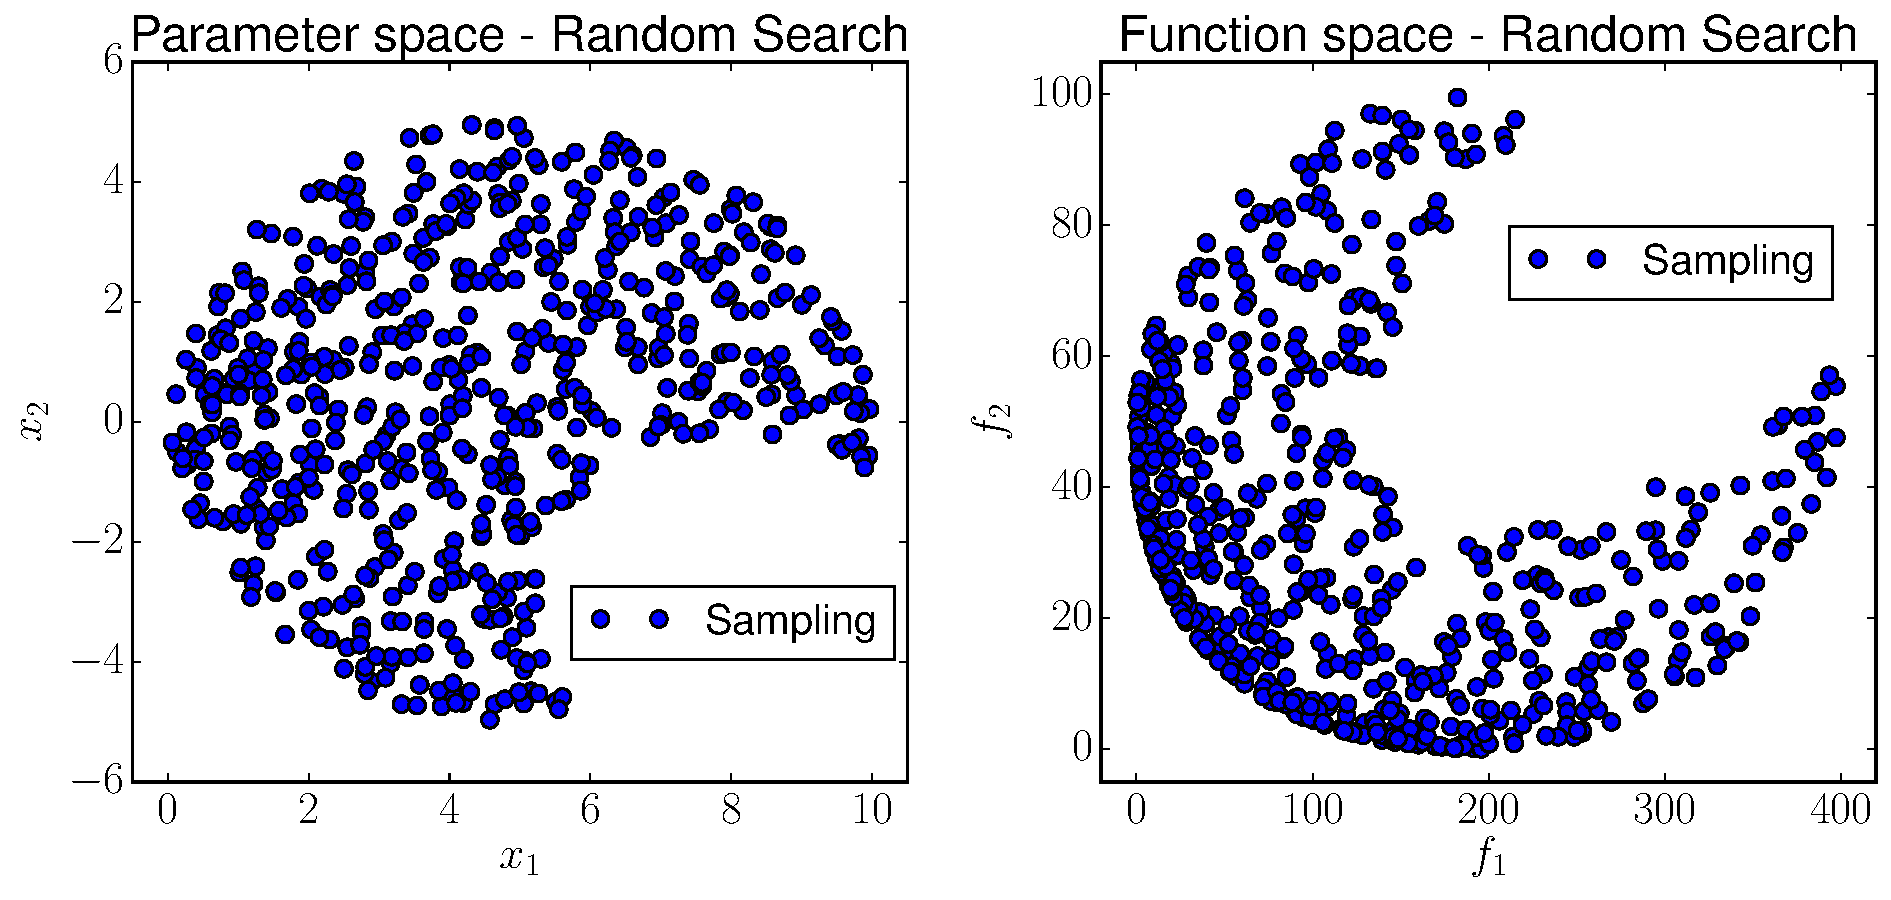
\includegraphics[width=0.85\textwidth]{Figures/3/mode_randomSearch.pdf}
        \caption{Random search method}
        \label{fig:randomSearch}
    \end{figure}
    \item General genetic algorithm: a general GA was coded up in Python. This GA may be used for a great variety of tasks and it is not designed for multiobjective optimization problems. Fitness is assigned with the distance to the Pareto front of each one of the individuals. The selection method chosen is the roulette method, with linear crossover and normal distribution mutation. The results obtained with this method show the Pareto front and how the individuals converge towards it along generations.     \begin{figure}[h!]
        \centering
        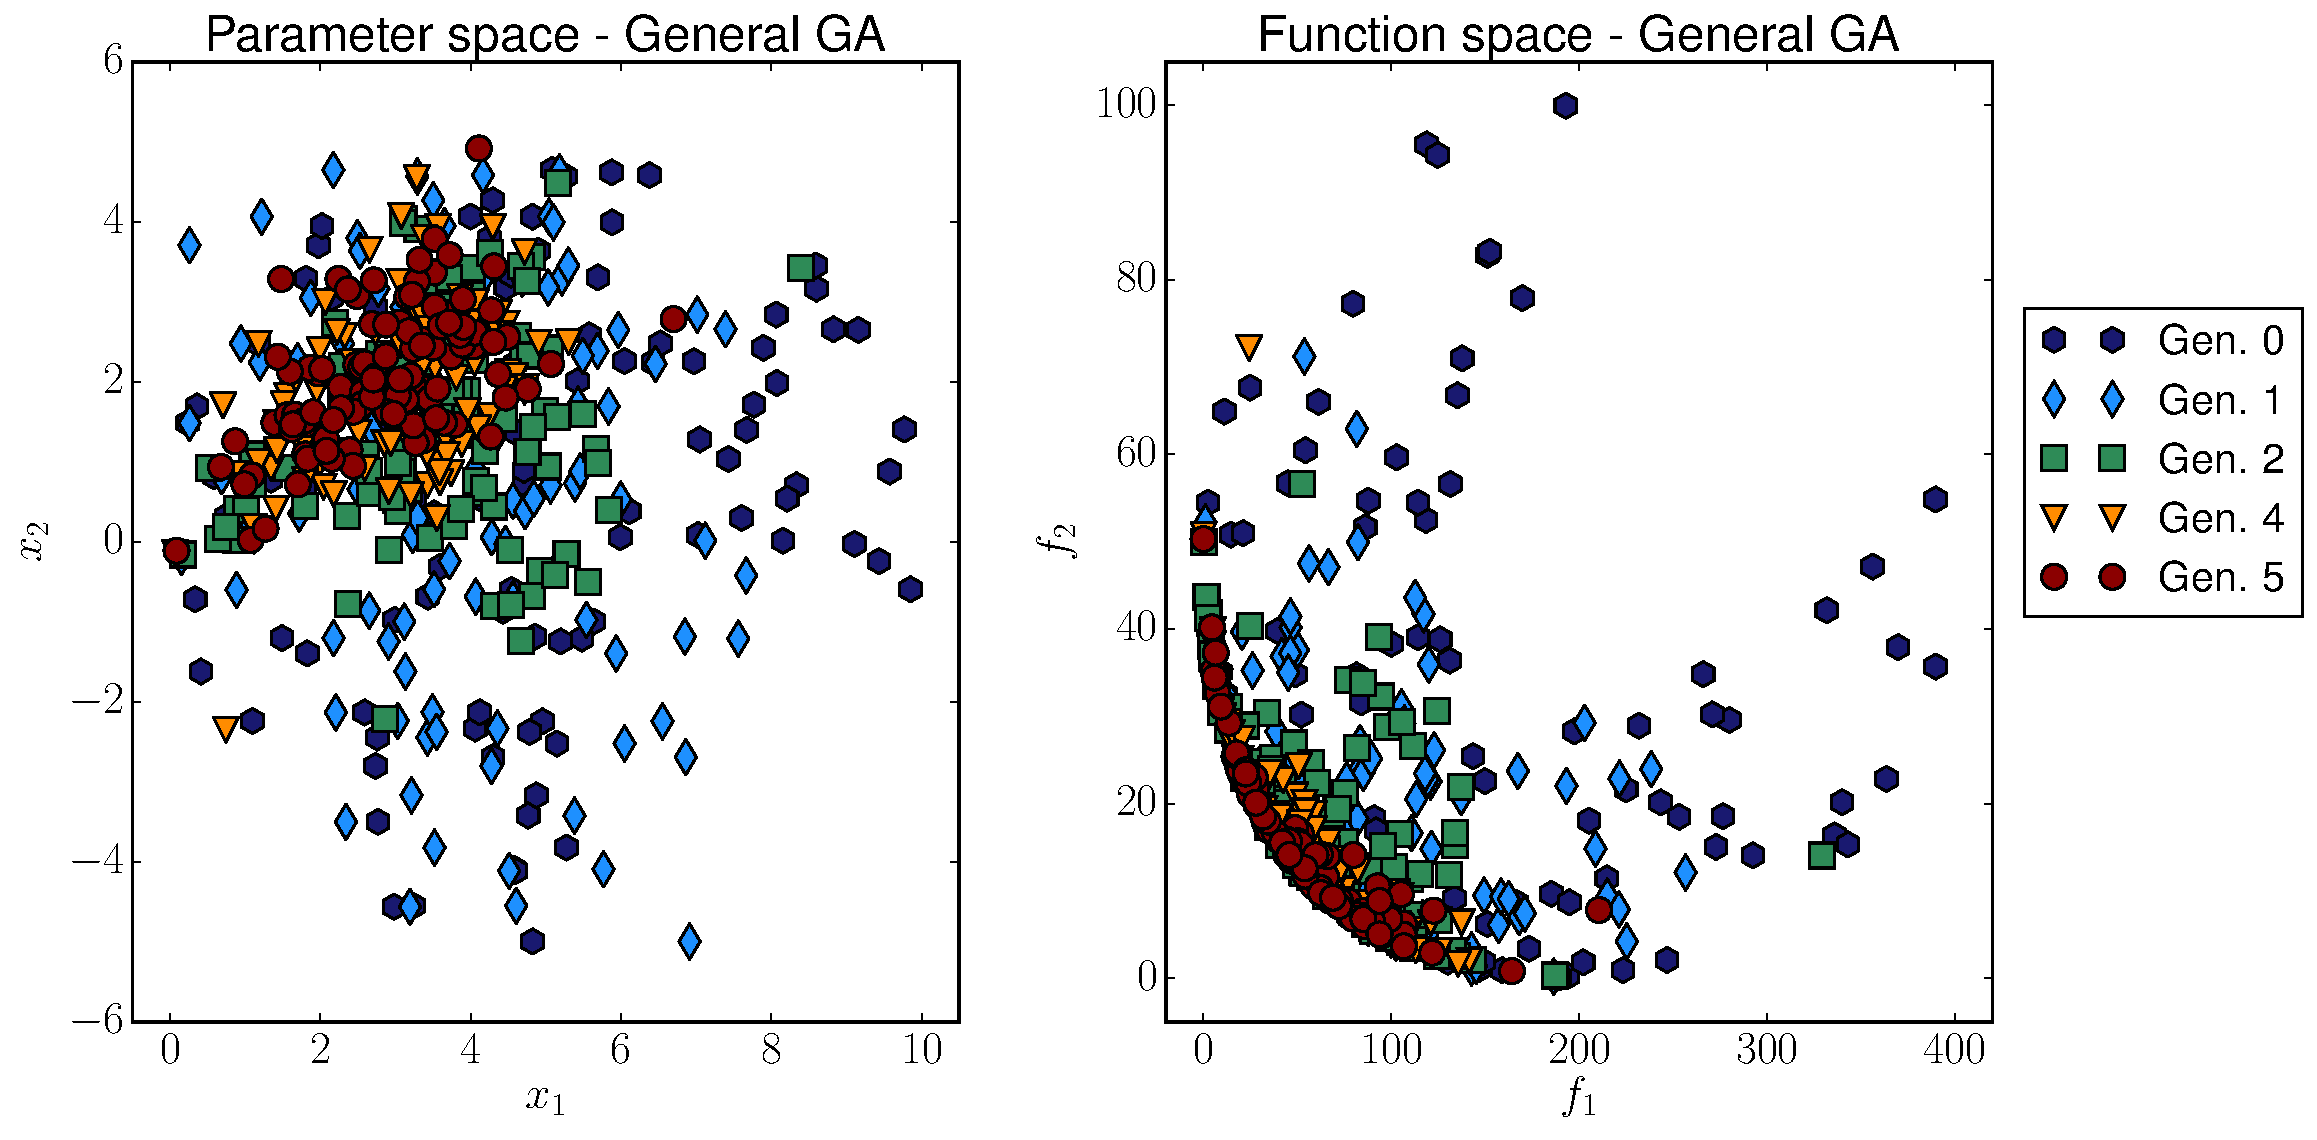
\includegraphics[width=0.8\textwidth]{Figures/3/mode_generalGAE.pdf}
        \caption{General genetic algorithm}
        \label{fig:plainGeneticAlgorithm}
    \end{figure}
    \item NSGA-II: the non-dominated sorting genetic algorithm is described in \cite{deb2002fast} and it is specially designed for multiobjective optimization problems. It is expected to have a greater convergence and more possibilities of capturing the whole Pareto front than the previously mentioned GA:
    \begin{figure}[h!]
        \centering
        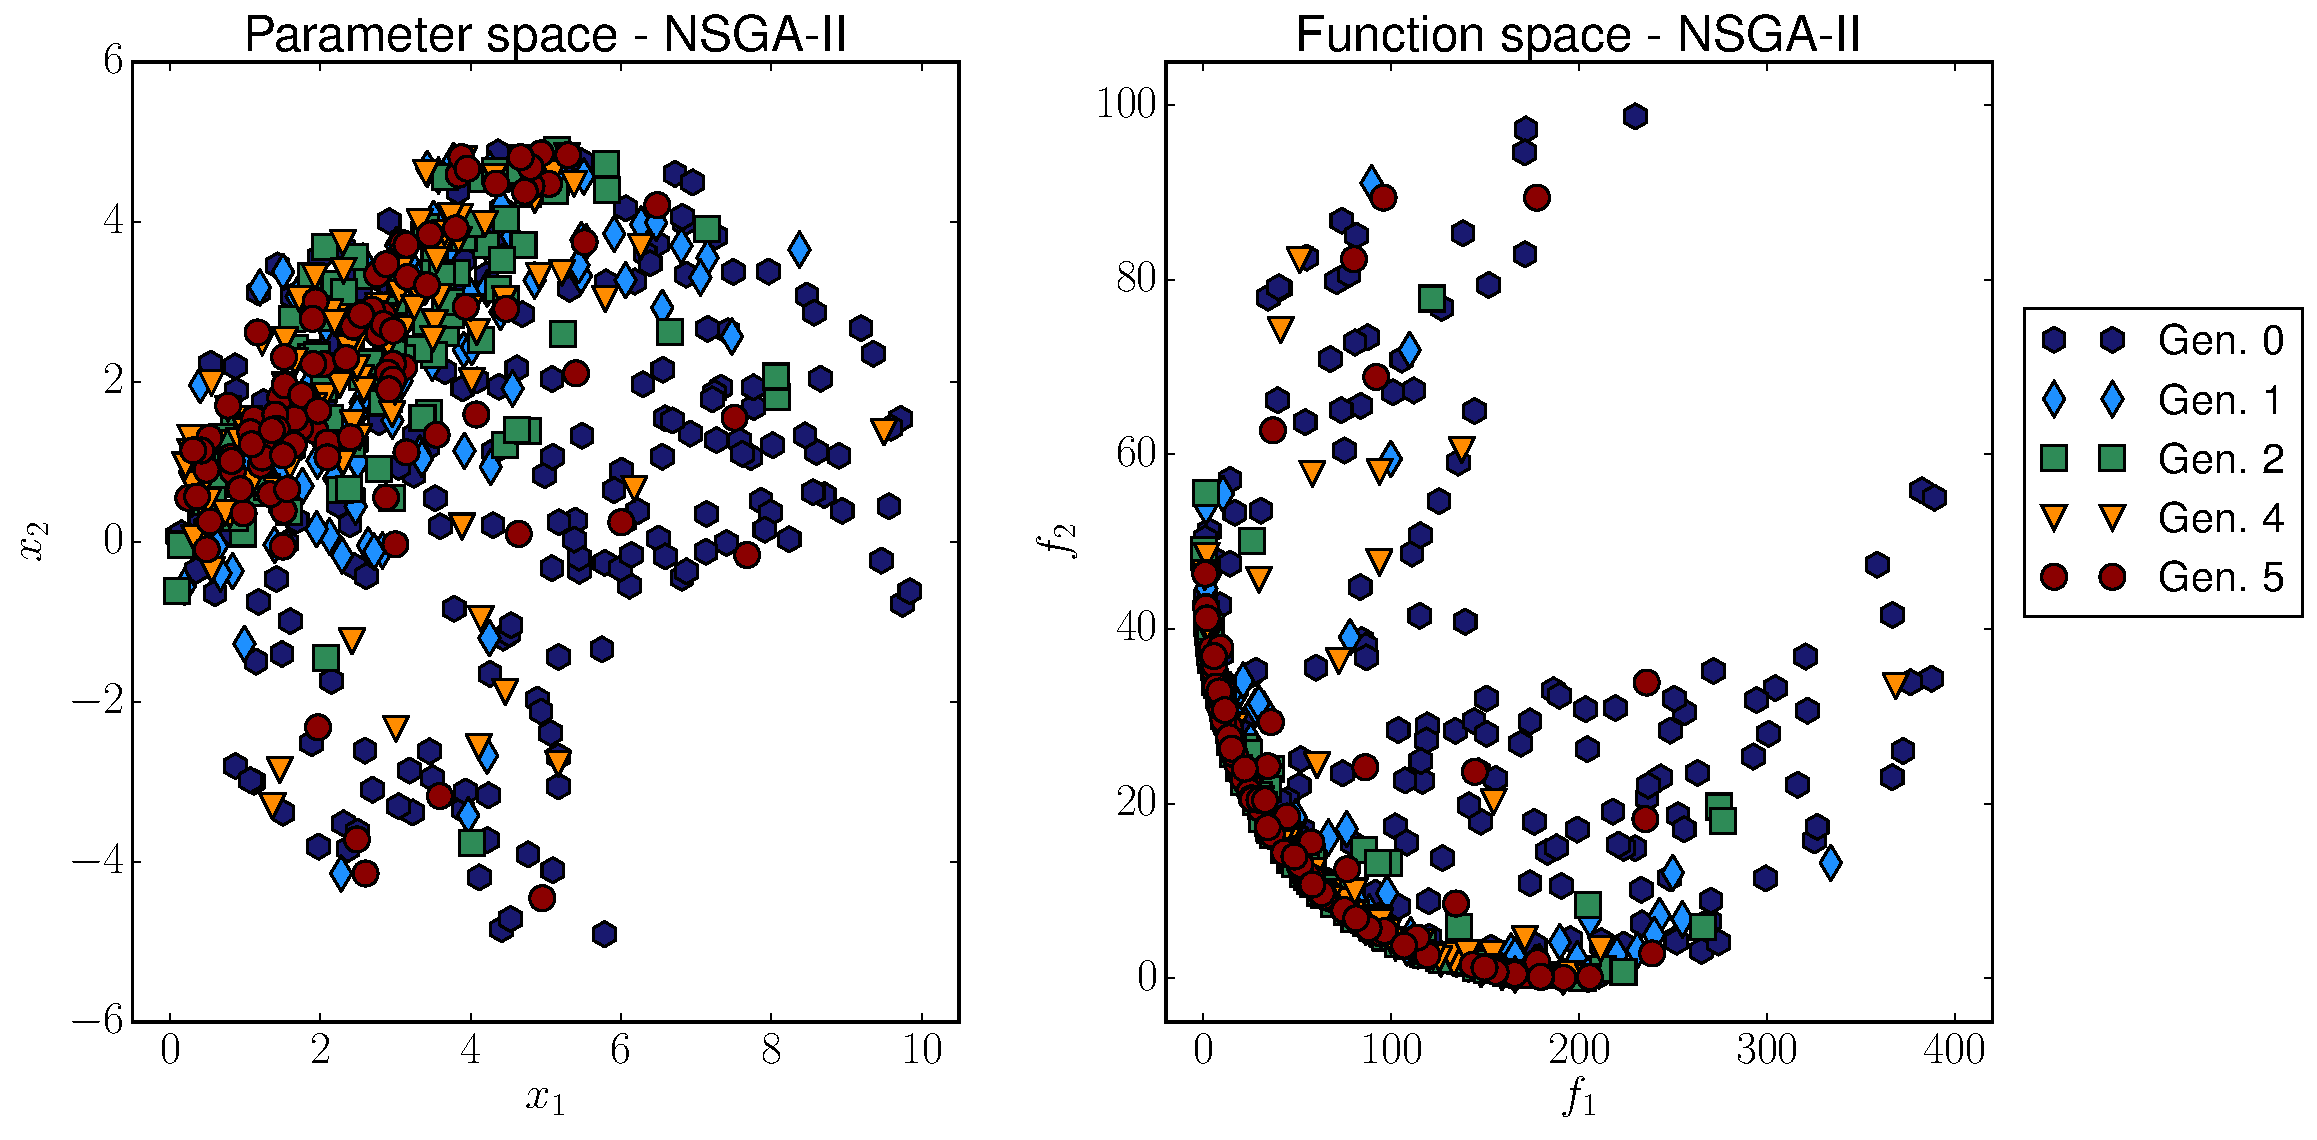
\includegraphics[width=0.8\textwidth]{Figures/3/mode_NSGA.pdf}
        \caption{Non-dominated sorted genetic algorithm II}
        \label{fig:NSGA-IIworkingMode}
    \end{figure}
\end{itemize}

\newpage

\subsection{Comparison of the performance of different methods}

The main question now is which one of these three methods will perform better, i.e., which one captures a more spread and precise Pareto front. The three methods searched the solution for different multiobjective optimization test functions, computing a histogram to show which is the probability of having an individual in certain area of the search and fitness spaces. Sixteen runs were performed, using the values shown in Table \ref{table:RSvsGAEvsNSGA}. It may be seen that the individuals in the random search are the same as the number of evaluations. Also for the general GA the number of individuals times the number of generations yields the number of evaluations. However, for the NSGA-II case, numbers don't add up at first glance because the first population of the NSGA-II is initialized with a population twice the size ($2N$) of the rest of the populations ($N$).

\begin{table}[H]
\centering
\renewcommand{\arraystretch}{1.1}
\caption{Different configurations for the different possibilities}
\label{table:RSvsGAEvsNSGA}
\begin{tabular}{|c|c|c|c|c|c|}
\hline
{\begin{tabular}[c]{@{}c@{}}RANDOM\\ SEARCH\end{tabular}} & \multicolumn{2}{c|}{{\begin{tabular}[c]{@{}c@{}}GENERAL\\ GA\end{tabular}}} & \multicolumn{2}{c|}{{NSGA-II}} & \multirow{2}{*}{{\begin{tabular}[c]{@{}c@{}}NUMBER OF \\ EVALUATIONS\end{tabular}}} \\ \cline{1-5}
{Indiv.} & {Indiv.} & {Gener.} & {Indiv.} & {Gener.} &  \\ \hline
80 & 10 & 8 & 10 & 7 & 80 \\ \hline
90 & 10 & 9 & 10 & 8 & 90 \\ \hline
100 & 10 & 10 & 10 & 9 & 100 \\ \hline
110 & 10 & 11 & 10 & 10 & 110 \\ \hline
200 & 25 & 8 & 25 & 7 & 200 \\ \hline
225 & 25 & 9 & 25 & 8 & 225 \\ \hline
250 & 25 & 10 & 25 & 9 & 250 \\ \hline
275 & 25 & 11 & 25 & 10 & 275 \\ \hline
450 & 50 & 9 & 50 & 8 & 450 \\ \hline
500 & 50 & 10 & 50 & 9 & 500 \\ \hline
550 & 50 & 11 & 50 & 10 & 550 \\ \hline
600 & 50 & 12 & 50 & 11 & 600 \\ \hline
900 & 100 & 9 & 100 & 8 & 900 \\ \hline
1000 & 100 & 10 & 100 & 9 & 1000 \\ \hline
1100 & 100 & 11 & 100 & 10 & 1100 \\ \hline
1200 & 100 & 12 & 100 & 11 & 1200 \\ \hline
\end{tabular}
\end{table}

Genetic algorithms are usually run for 25000 iterations, with populations of 250 individuals. However, here the number of function evaluations is way lower because when applied to CFD, several minutes will take the evaluation of each individual (whereas for a function optimization, a whole population evaluation may last seconds).

\newpage

The test functions used were:
\begin{itemize}
\item \textbf{Bihn \& Korn test function:} this function was already described before (\ref{eq:BihnKorn}) but it is added here again for clarification. This is a function-constrained search optimization, with two objectives and two variables:
    \begin{equation}
        \begin{array}{cl}
            \textrm{minimize} & 
            \left\{ \begin{array}{l}
                f_1(x_1,x_2) = 4x_1^2 + 4x_2^2\\
                f_2(x_1,x_2) = (x_1-5)^2+(x_2-5)^2
            \end{array} \right. \\
            & \\
            \textrm{subject to} &  
            \left\{ \begin{array}{l}
                (x_1-5)^2+x_2^2-25 \leq 0\\
                -(x_1-8)^2-(x_2+3)^2 + 7.7 \leq 0
            \end{array} \right. \\
            & \\
            \textrm{bounded by} & -15 \leq x_i \leq 30, \ \ \forall i = 1,2
        \end{array}
        \tag{\ref{eq:BihnKorn} revisited}
    \end{equation}

\item \textbf{Poloni's test function:} two objectives and two variables test function \cite{poloni1995hybrid}:
    \begin{equation}
\begin{array}{cl}
            \textrm{minimize} & 
            \left\{ \begin{array}{l}
                f_1(x_1,x_2) = 1+\left[A_1-B_1(x_1,x_2)\right]^2+\left[A_2-B_2(x_1,x_2)\right]^2\\
                f_2(x_1,x_2) = (x_1+3)^2+(x_2+1)^2
            \end{array} \right. \\
            & \\
            \textrm{where} & 
            \left\{ \begin{array}{l}
                A_1 = 0.5\sin(1)-2\cos(1)+\sin(2)-1.5\cos(2) \\
                A_2 = 1.5\sin(1)-\cos(1)+2\sin(2)-0.5\cos(2) \\
                B_1(x_1,x_2) = 0.5\sin(x_1)-2\cos(x_1)+\sin(x_2)-1.5\cos(x_2) \\
                B_2(x_1,x_2) = 1.5\sin(x_1)-\cos(x_1)+2\sin(2)-0.5\cos(x_2)
            \end{array} \right. \\
            & \\
            \textrm{in} & -\pi \leq x_i \leq \pi, \ \ \forall i = 1,2
        \end{array}
        \label{eq:poloni}
    \end{equation}

\item \textbf{Zitzler-Deb-Thiele's test functions:} ZDT are a classical set of test functions designed for genetic algorithms to test its performance. They are designed for 30 variables and bi-objective optimization, but in this case, the ZDT2 function was adapted to just two variables in the search space \cite{zitzler2000comparison}:
    \begin{equation}
\begin{array}{cl}
            \textrm{minimize} & 
            \left\{
             \arraycolsep=1.0pt\def\arraystretch{2.0} \begin{array}{l}
            f_1(x_1,x_2) = x_1\\
            f_2(x_1,x_2) = g(x_1,x_2) \cdot h(f_1(x_1,x_2),g(x_1,x_2))\\
            g(x_1,x_2) = 1+\dfrac{9x_2}{29} \\
            h(x_1,x_2) = 1 - \sqrt{\dfrac{x_1}{x_2}}
            \end{array} \right. \\
            & \\
           \textrm{bounded by} & 0 \leq x_i \leq 1, \ \ \forall i = 1,2
        \end{array}
        \label{eq:ZDT2}
    \end{equation}
\end{itemize}

\newpage

    \begin{figure}[H]
        \centering
        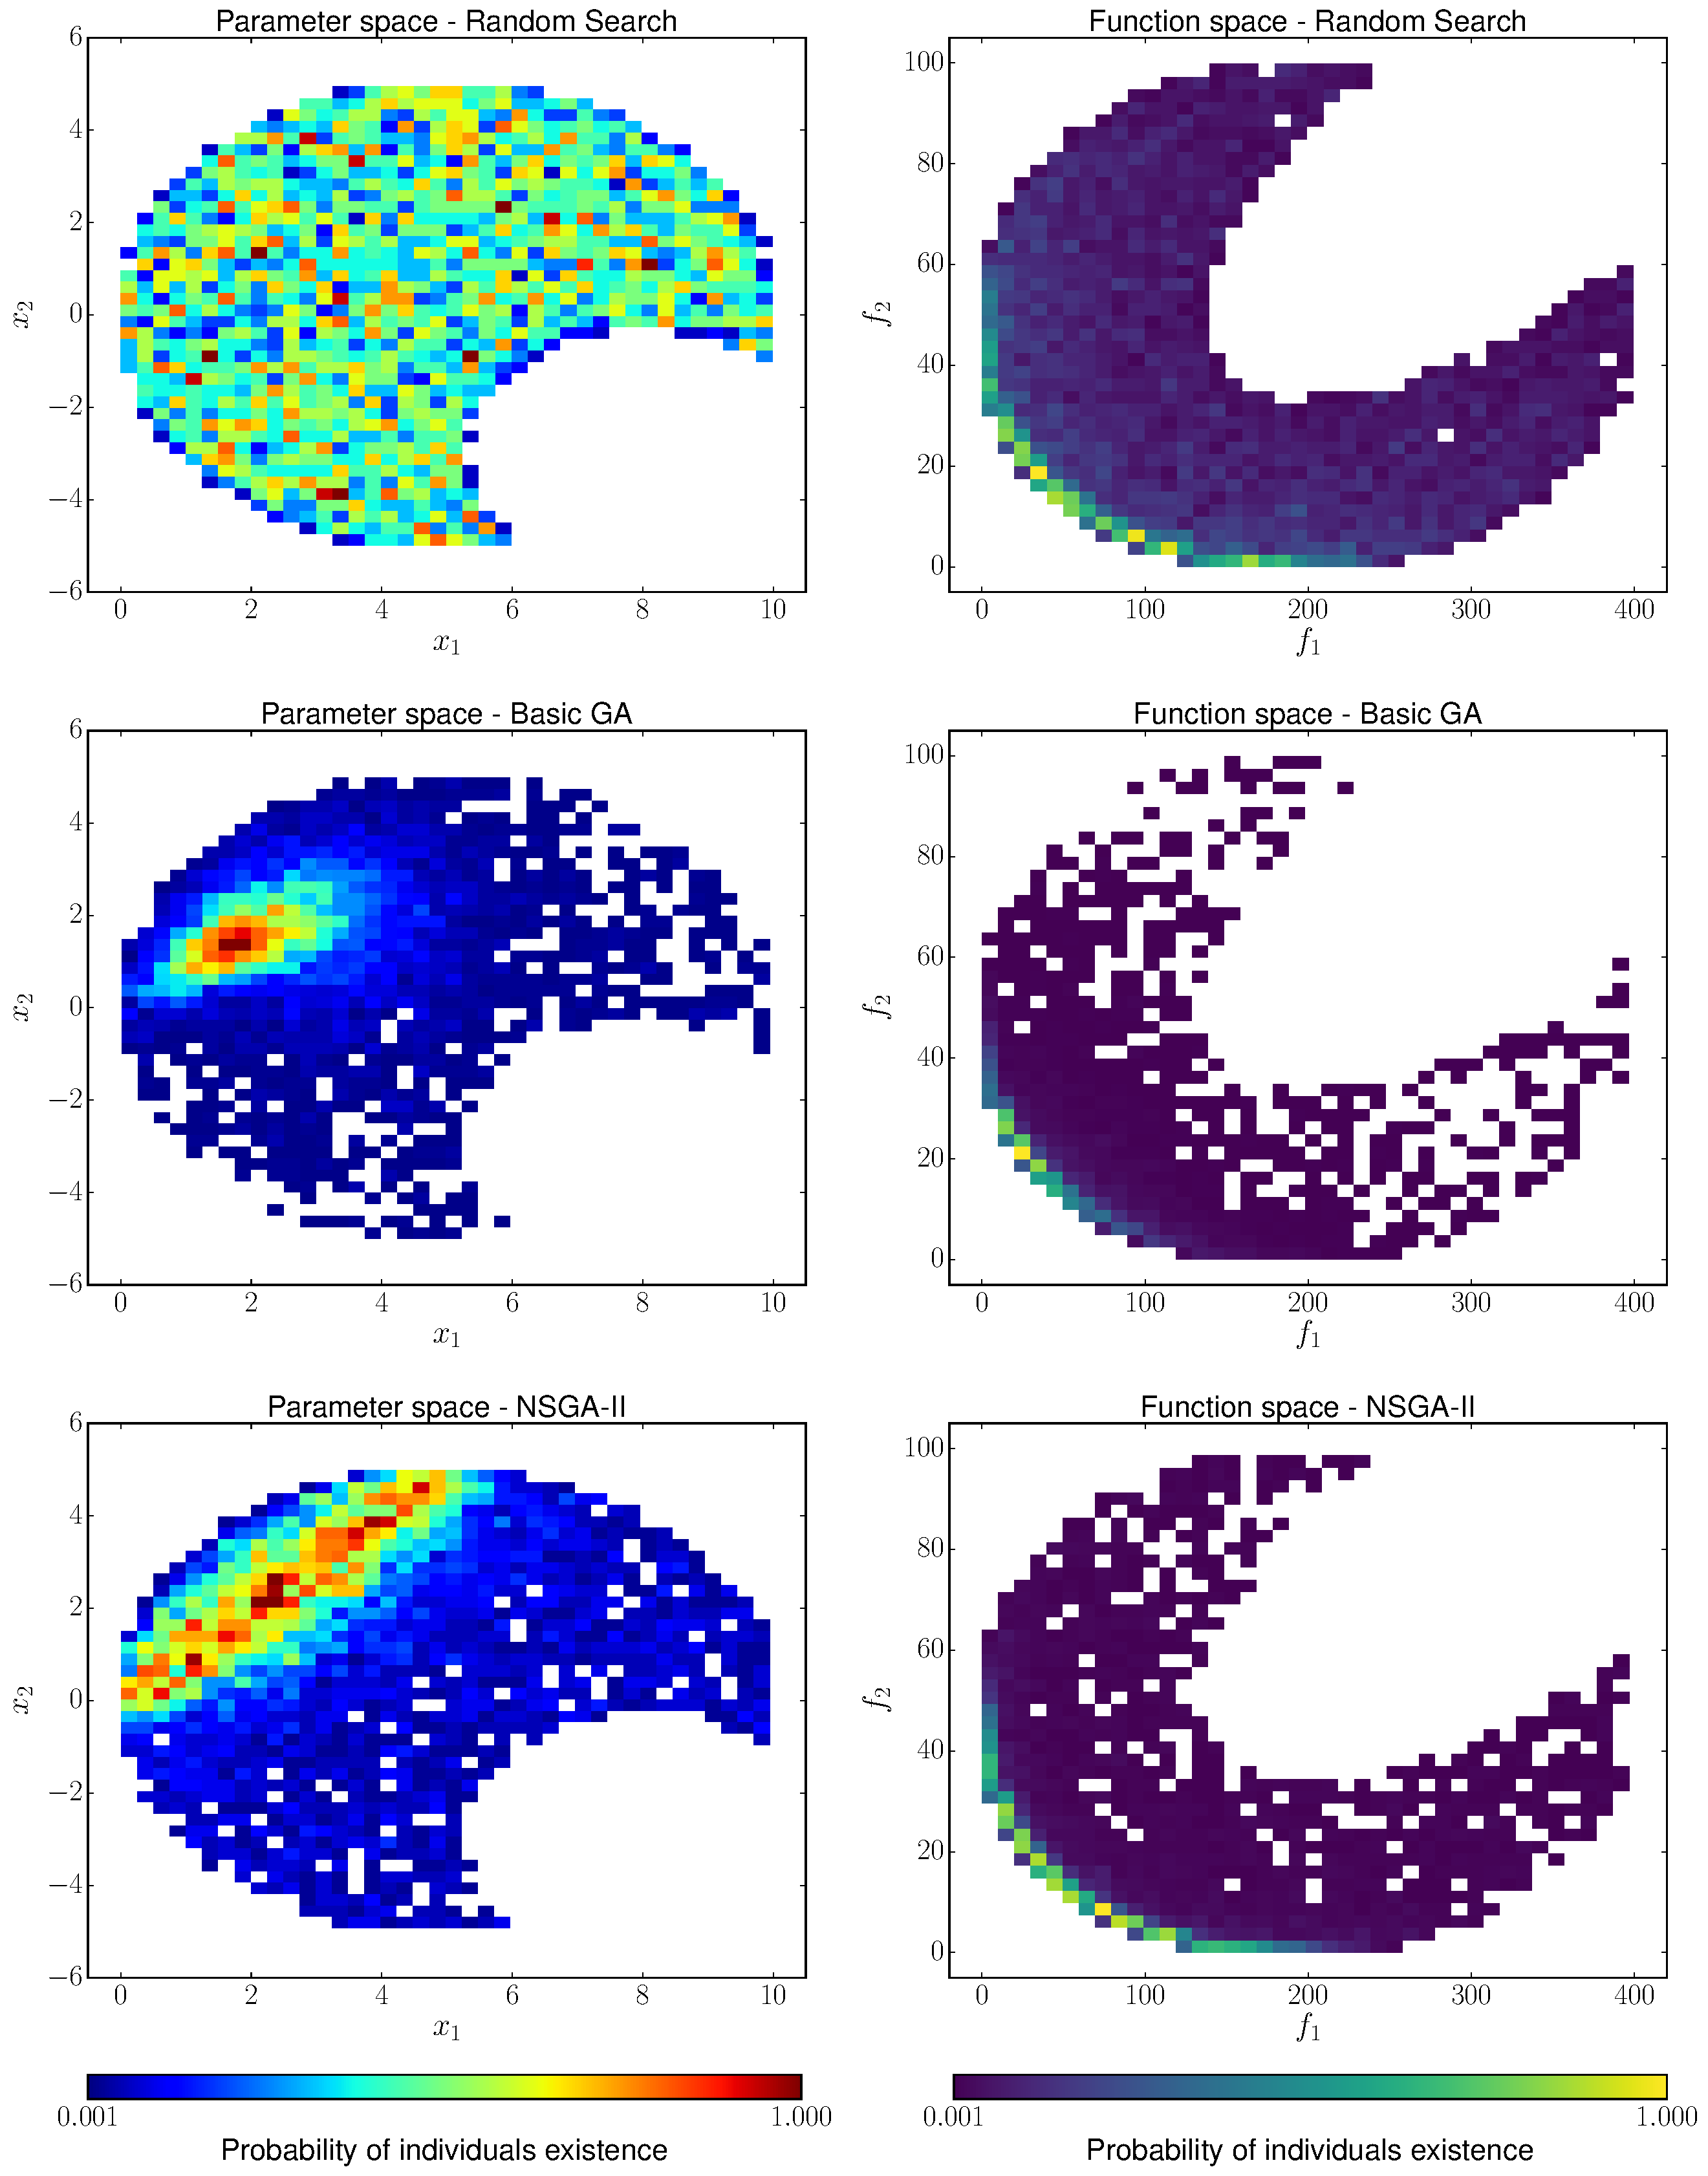
\includegraphics[height=0.96\textheight, width=\textwidth]{Figures/3/hist_BK.pdf}
        \caption{Method comparison for the Bihn \& Korn function}
        \label{fig:histogramBK}
    \end{figure}
    
\newpage

    \begin{figure}[H]
        \centering
        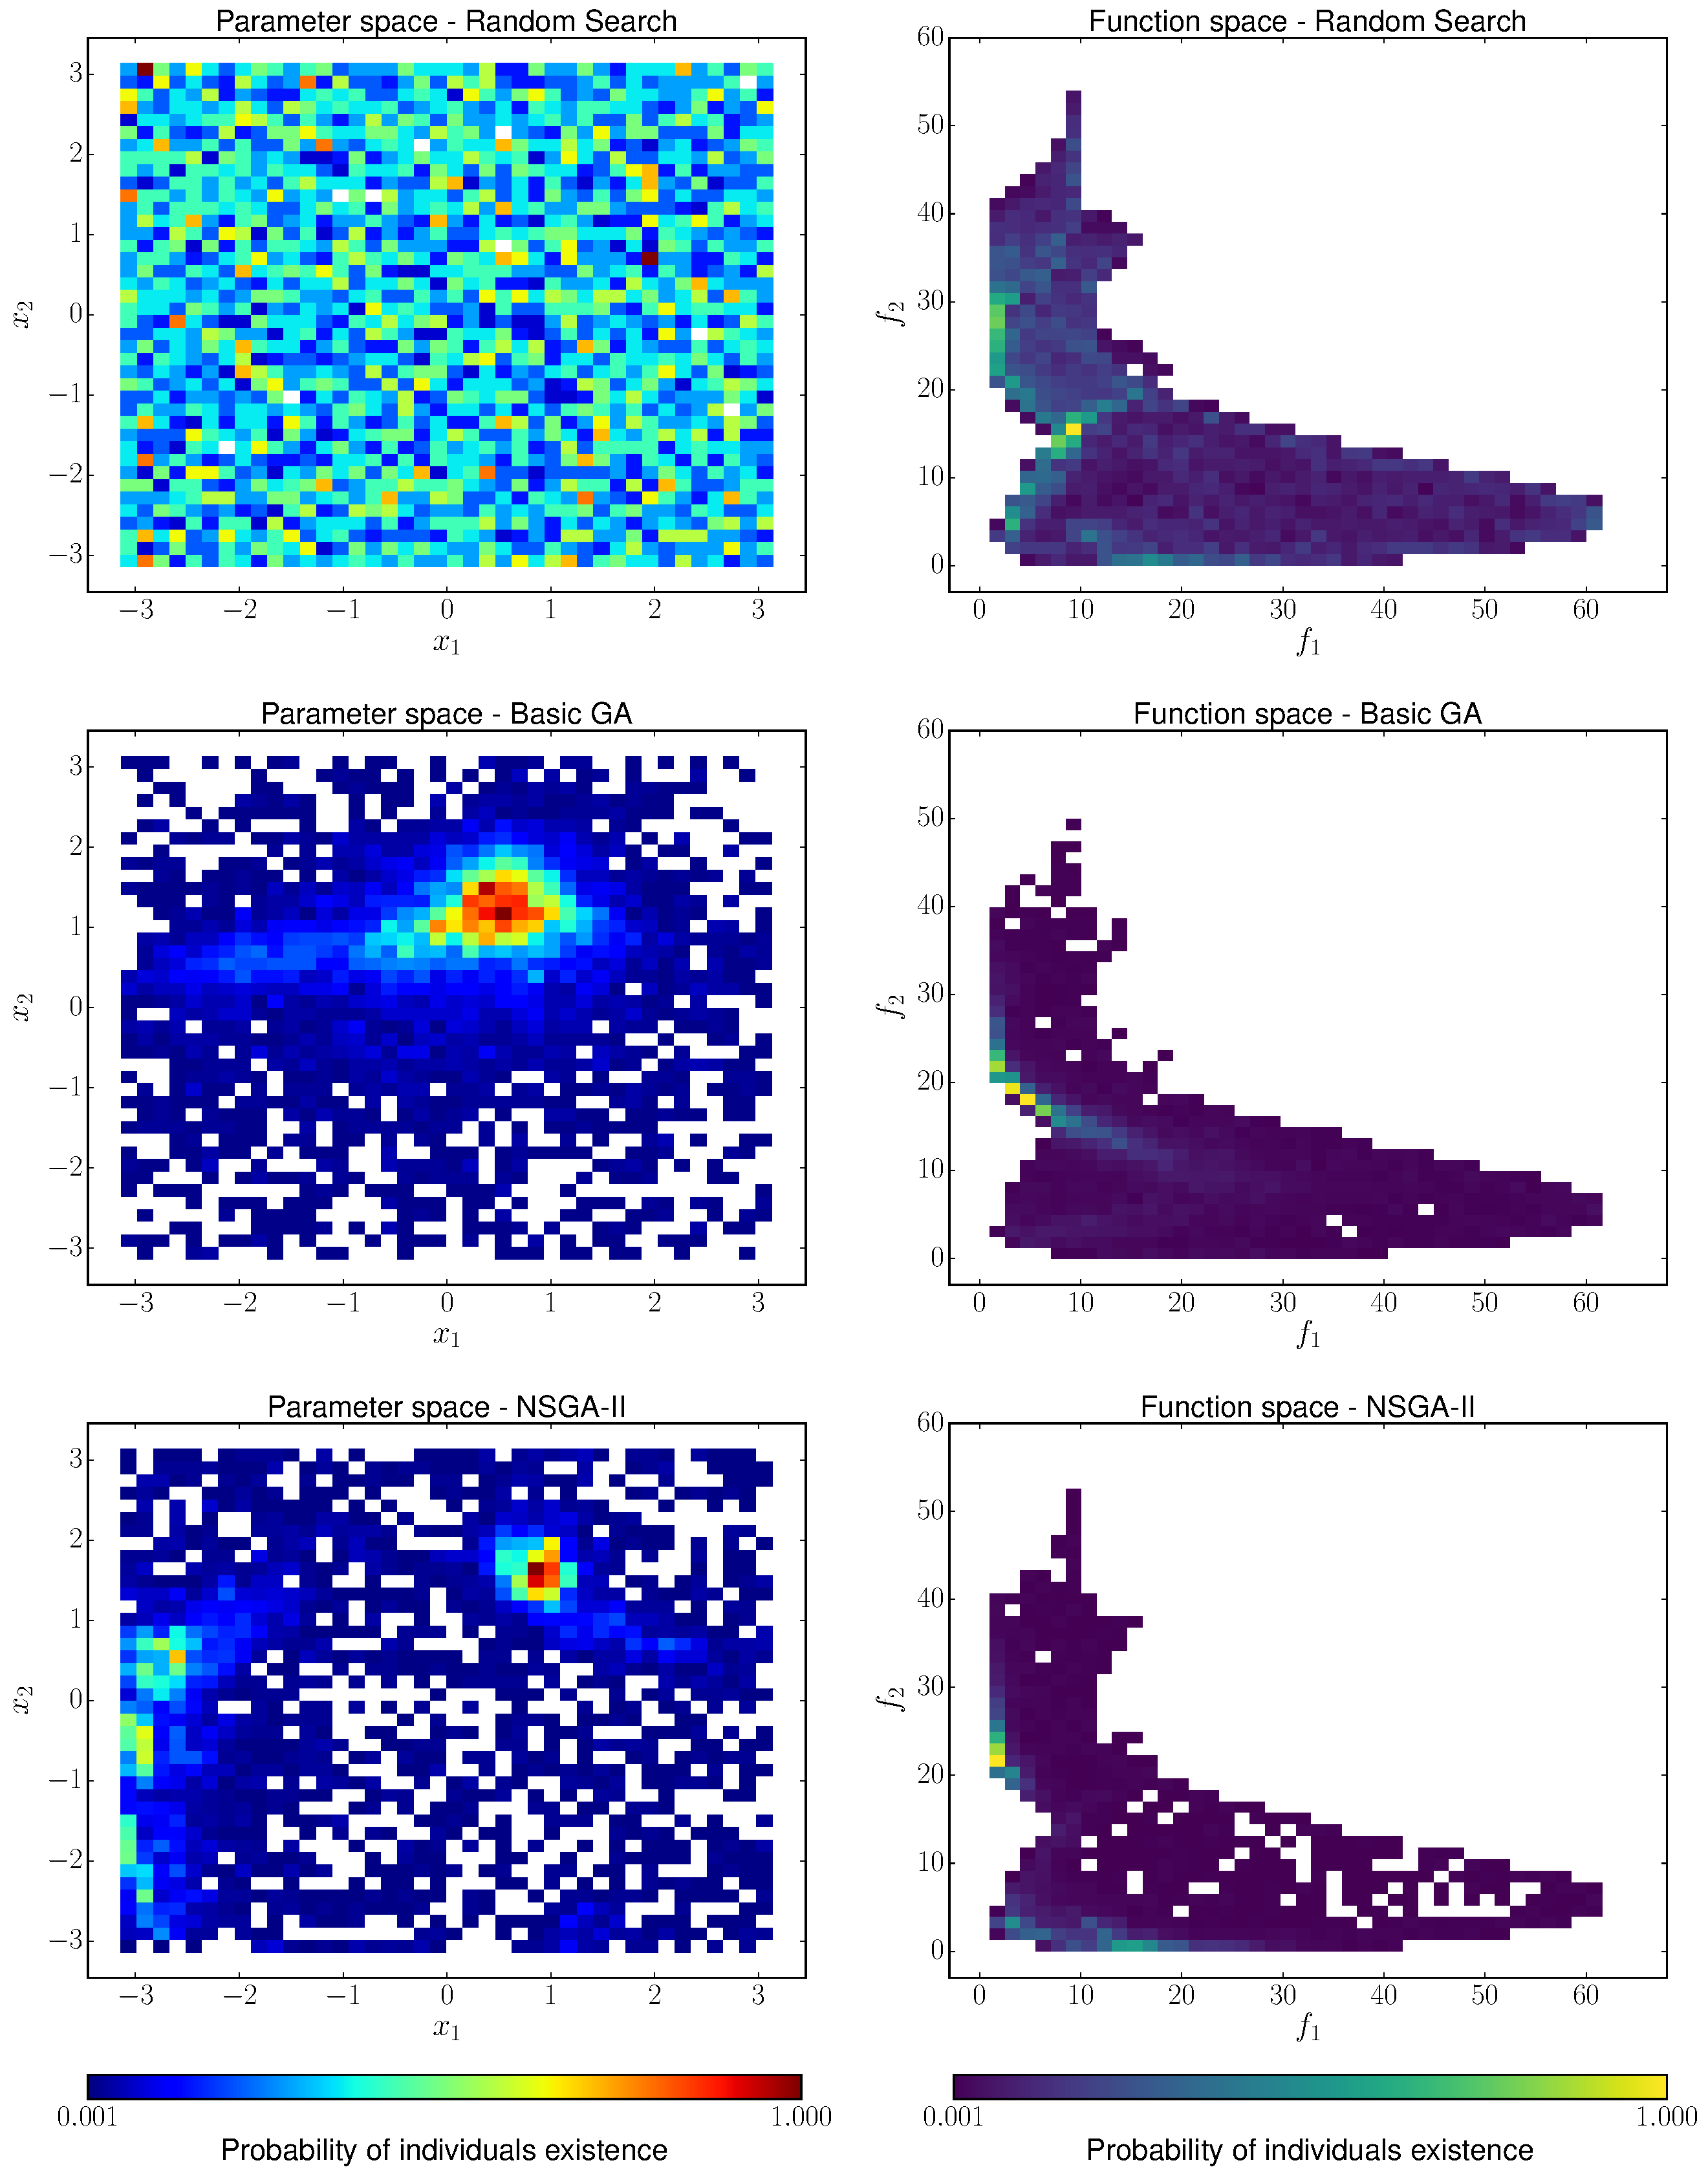
\includegraphics[height=0.96\textheight, width=\textwidth]{Figures/3/hist_POL.pdf}
        \caption{Method comparison for the Poloni's function}
        \label{fig:histogramPOL}
    \end{figure}
    
\newpage

    \begin{figure}[H]
        \centering
        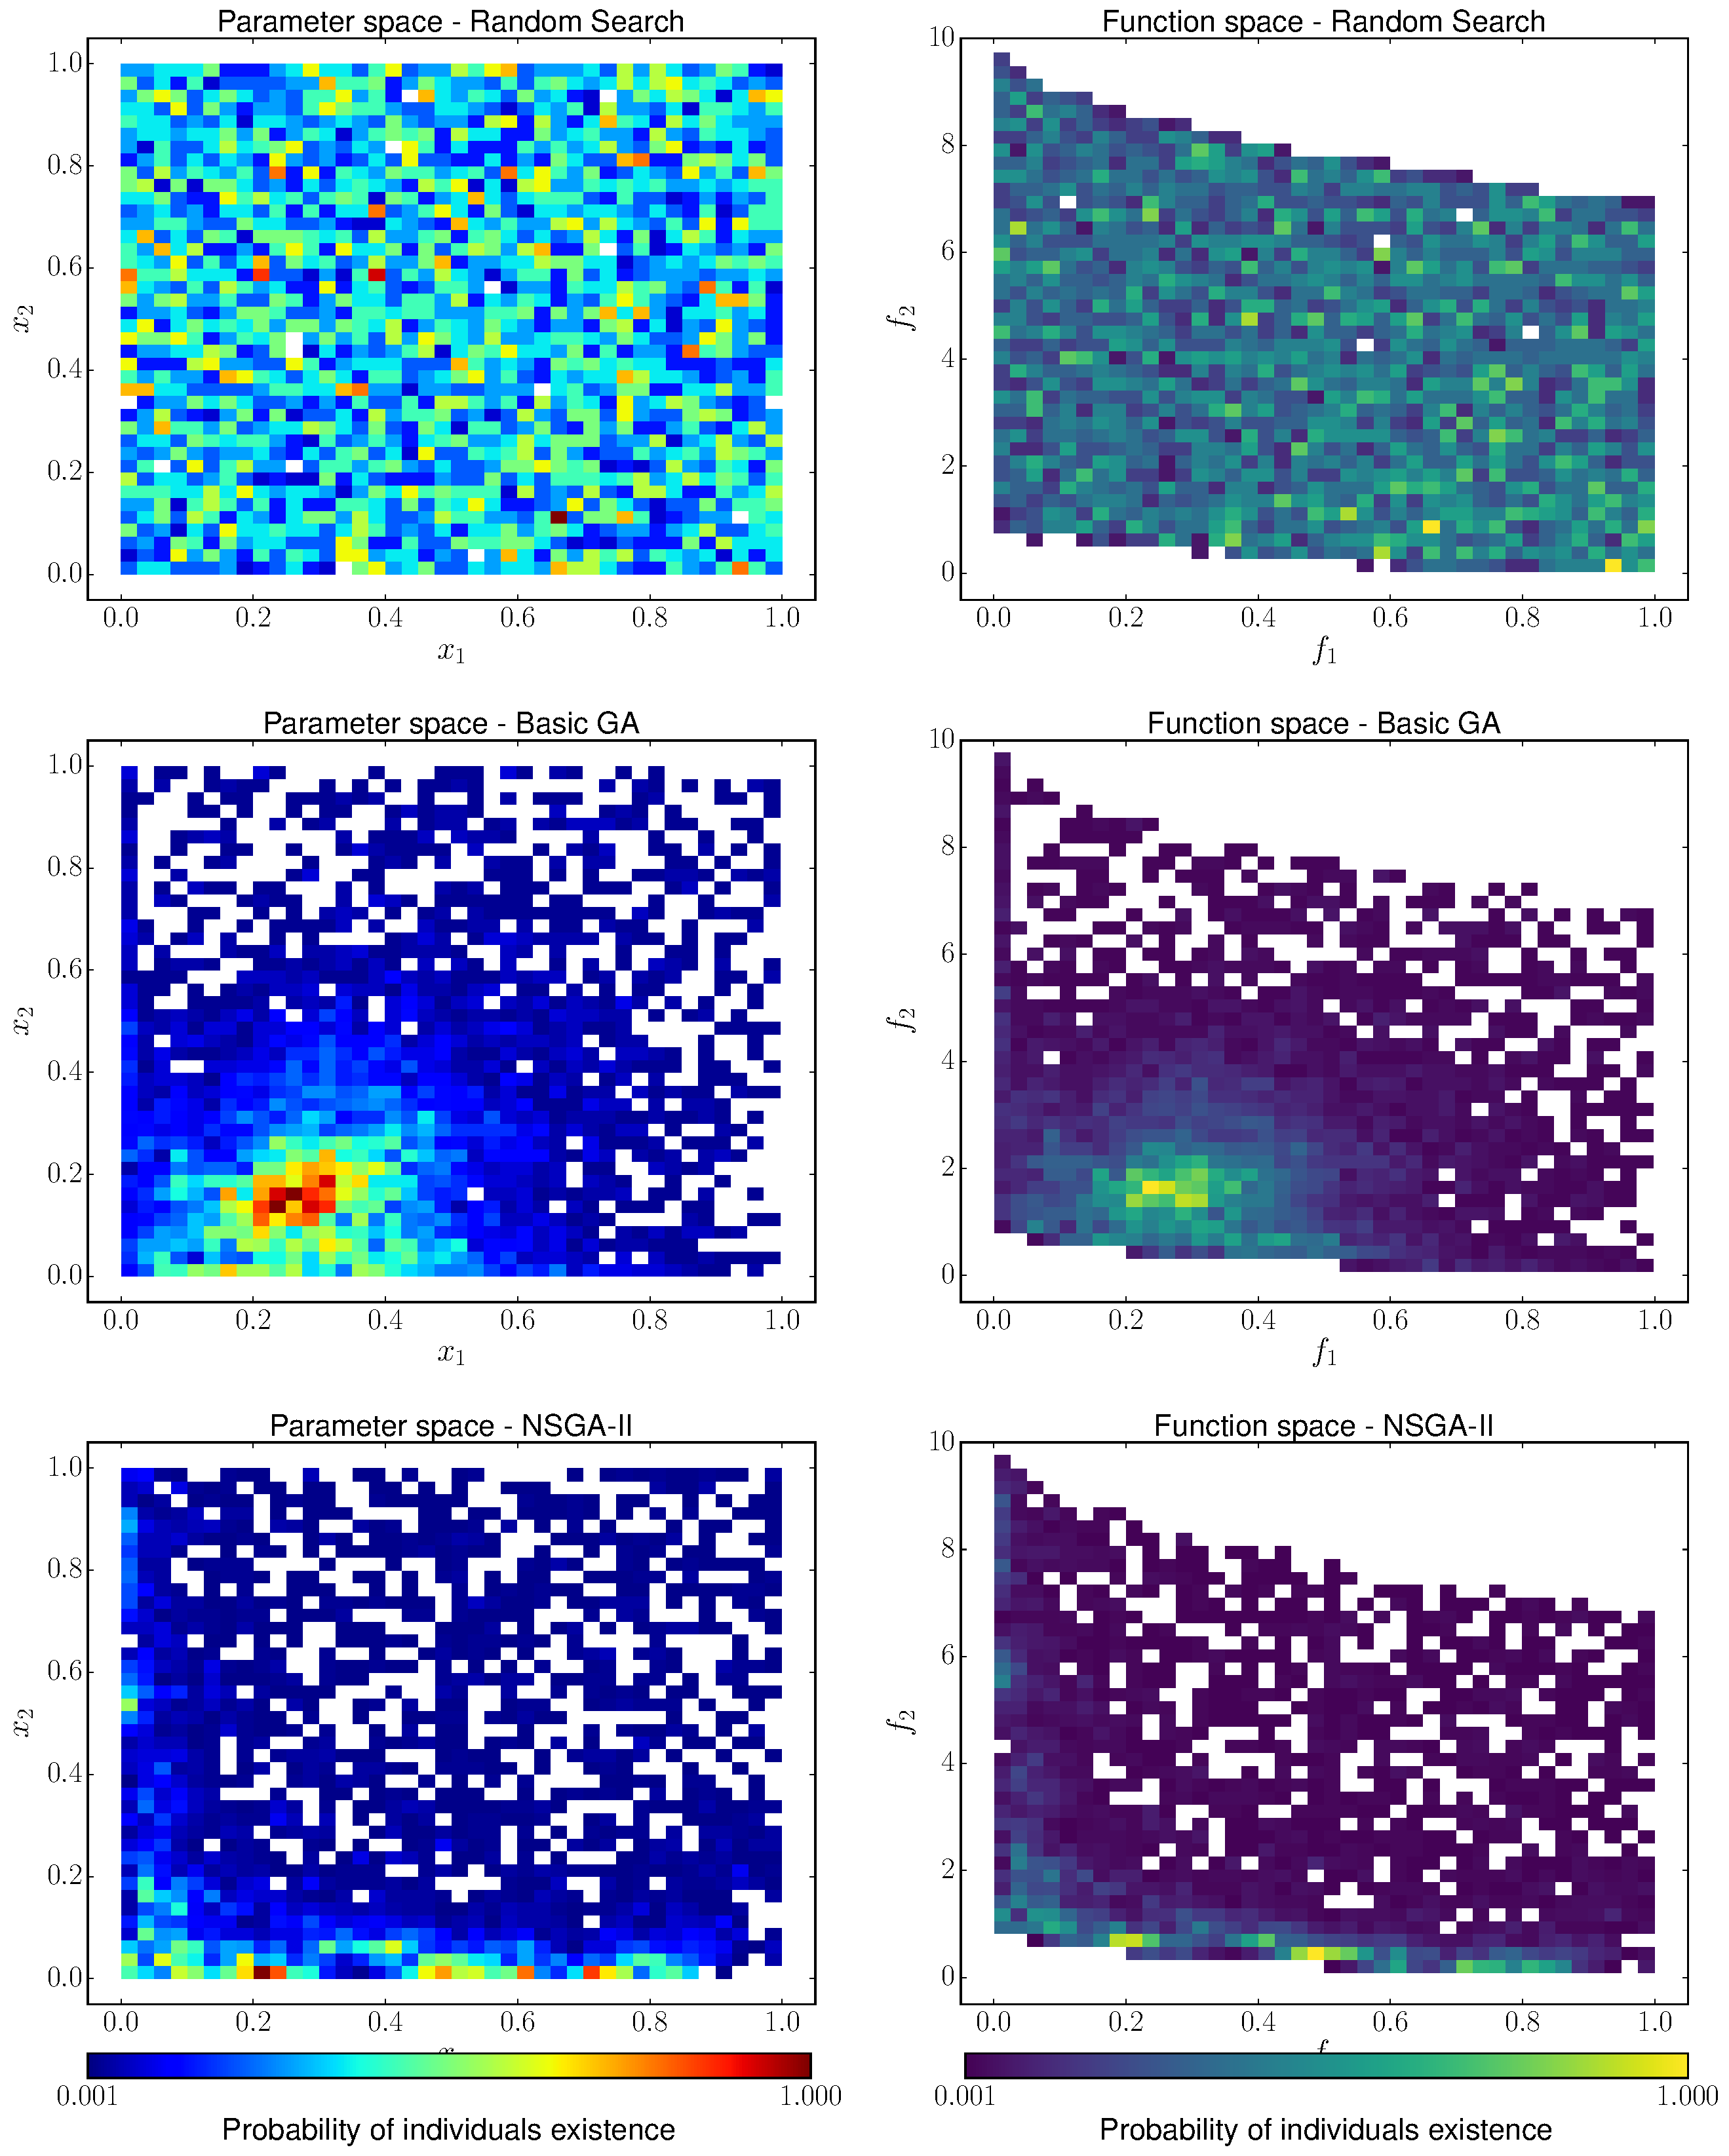
\includegraphics[height=0.96\textheight, width=\textwidth]{Figures/3/hist_ZDT2.pdf}
        \caption{Method comparison for the ZDT2 function}
        \label{fig:histogramZDT2}
    \end{figure}
    
\newpage

It can be seen that for the three functions, the random search cover the whole parameter space uniformly. However, this does not mean that the function space is better analyzed in the surroundings of the Pareto front (see Figure \ref{fig:histogramZDT2}). Thus the random search is not valid even for a two variable case because it does not converge nor evolve towards a solution. The basic GA and the NSGA-II points converge to certain areas, although the basic GA does not cover the whole Pareto front as it should (see Figure \ref{fig:histogramPOL}) or does not capture it at all (see Figure \ref{fig:histogramZDT2}). Thus the only method that is really valid for searching in complex parameter spaces and converge to a true Pareto front is the NSGA-II (see Figures \ref{fig:histogramBK}, \ref{fig:histogramPOL} and \ref{fig:histogramZDT2}). Although this comparison may be seen biased for the different algorithms, the optimization in CFD is usually performed with Monte Carlo methods which are a random search that may not be the most effective methods. 

\subsection{Number of evaluations versus number of generations}

Given that NSGA-II is the algorithm chosen for solving multiobjective optimization problems, a deep knowledge of how the dynamics of the system really work is essential to achieve an accurate solution. The NSGA-II depends only on two variables, which are the number of individuals per generation and the limit in the number of generations. The same number of function evaluations (translated in the future to CFD simulations) may be distributed in different combinations of individuals and generations. In order to prove if it is better to have more individuals or generations (for the same number of function evaluations) two measures proposed by \cite{deb2002fast} are used:
\begin{itemize}
    \item Diversity metric ($\Delta$): it measures the extent of spread achieved in the solutions by taking the distance between each one of the points that form the Pareto-optimal front. The best value will be zero, having that all individuals are at the same distance one to each other. This metric is only valid for bi-objective optimization, but a Voronoi triangularization may be used for Pareto front in higher dimensions: 
    \begin{equation}
        \displaystyle \Delta = \dfrac{d_f+d_l+\sum^{N-1}_{i=1}|d_i-\bar{d}|}{d_f+d_l+(N-1)\bar{d}}
    \end{equation}
\item Convergence metric ($\Upsilon$): this metric may only be used in cases where the Pareto front may be known, because it is defined as the minimum distance to the true Pareto front ($\mathcal{PF}_0$):
\begin{equation}
    \Upsilon =  \text{min} (\text{dist}({PF_{GA}}_i,\mathcal{PF}_0)) 
\end{equation}
\end{itemize}


\newpage

The three test functions described before (\ref{eq:BihnKorn}, \ref{eq:poloni} and \ref{eq:ZDT2}) are used again as a way of knowing how the algorithm really behaves. They were tested with all the cases shown in the Table \ref{table:nubmerofgen}, running each one of the possible configurations 20 times in order to capture the dynamics of the configurations.

\begin{table}[H]
\centering
\renewcommand{\arraystretch}{1.6}
\caption{Generations and individuals combinations tested for performance}
\label{table:nubmerofgen}
\begin{tabular}{c|c|c|c|c|c}
\cline{2-6}
 & \multicolumn{5}{c|}{\textbf{INDIVIDUALS PER GENERATION}} \\ \hline
\multicolumn{1}{|c|}{\textbf{\begin{tabular}[c]{@{}c@{}}TOTAL FUNCTION\\ EVALUATIONS\end{tabular}}} & \textbf{8} & \textbf{16} & \textbf{32} & \textbf{64} & \multicolumn{1}{c|}{\textbf{128}} \\ \hline
\multicolumn{1}{|c|}{\textbf{640}} & 79 & 39 & 19 & 9 & \multicolumn{1}{c|}{4} \\ \hline
\multicolumn{1}{|c|}{\textbf{512}} & 63 & 31 & 15 & 7 & \multicolumn{1}{c|}{3} \\ \hline
\multicolumn{1}{|c|}{\textbf{384}} & 47 & 23 & 1 & 5 & \multicolumn{1}{c|}{2} \\ \hline
\multicolumn{1}{|c|}{\textbf{256}} & 31 & 15 & 7 & 3 & \multicolumn{1}{c|}{\textit{(trivial)}} \\ \hline
\multicolumn{1}{|c|}{\textbf{128}} & 15 & 7 & 3 & \textit{(trivial)} &  \\ \cline{1-5}
\end{tabular}
\end{table}

As said before, it must be noted that the first generation of the NSGA-II has twice the size of the rest of populations. This also created some \textit{trivial} cases, because if the number of individuals is $N$ and the total function evaluations are fixed to be $2N$, the first population will cover all the possible function evaluations (so it will be a random search and not an evolutionary computation algorithm). 

The values shown in the figures are the mean and standard deviation of the two metrics, having that Figure \ref{fig:diverMetric} has error bars with the mean ($\mu_\Delta$) and standard deviation ($\sigma_\Delta$) of the analyzed cases, while the error bars in Figure \ref{fig:convMetric} represent $\mu_\Upsilon$ and $\sigma_\Upsilon$. The values are very high when compared with the ones obtained in \cite{deb2002fast} for the same test functions, but as said before the number of function evaluations is very low when compared to those in the paper.  

The results in Figure \ref{fig:diverMetric} for the divergence metric ($\Delta$) show not conclusive results. There is not a clear trend seen in all three functions. The vertical axis has the same limit in all subfigures in order to compare more easily the results. Although it may seem that for a small number of generations the metric has a higher value (having that the best approach will be to have a greater number of generations), the changes are slight and they do not serve to draw any conclusion. It is interesting to see that the Bihn \& Korn function yield the same results without any dependence on the combination (reducing only the standard deviation with more evaluations).

    \newpage
    
    \begin{figure}[h!]
        \centering
        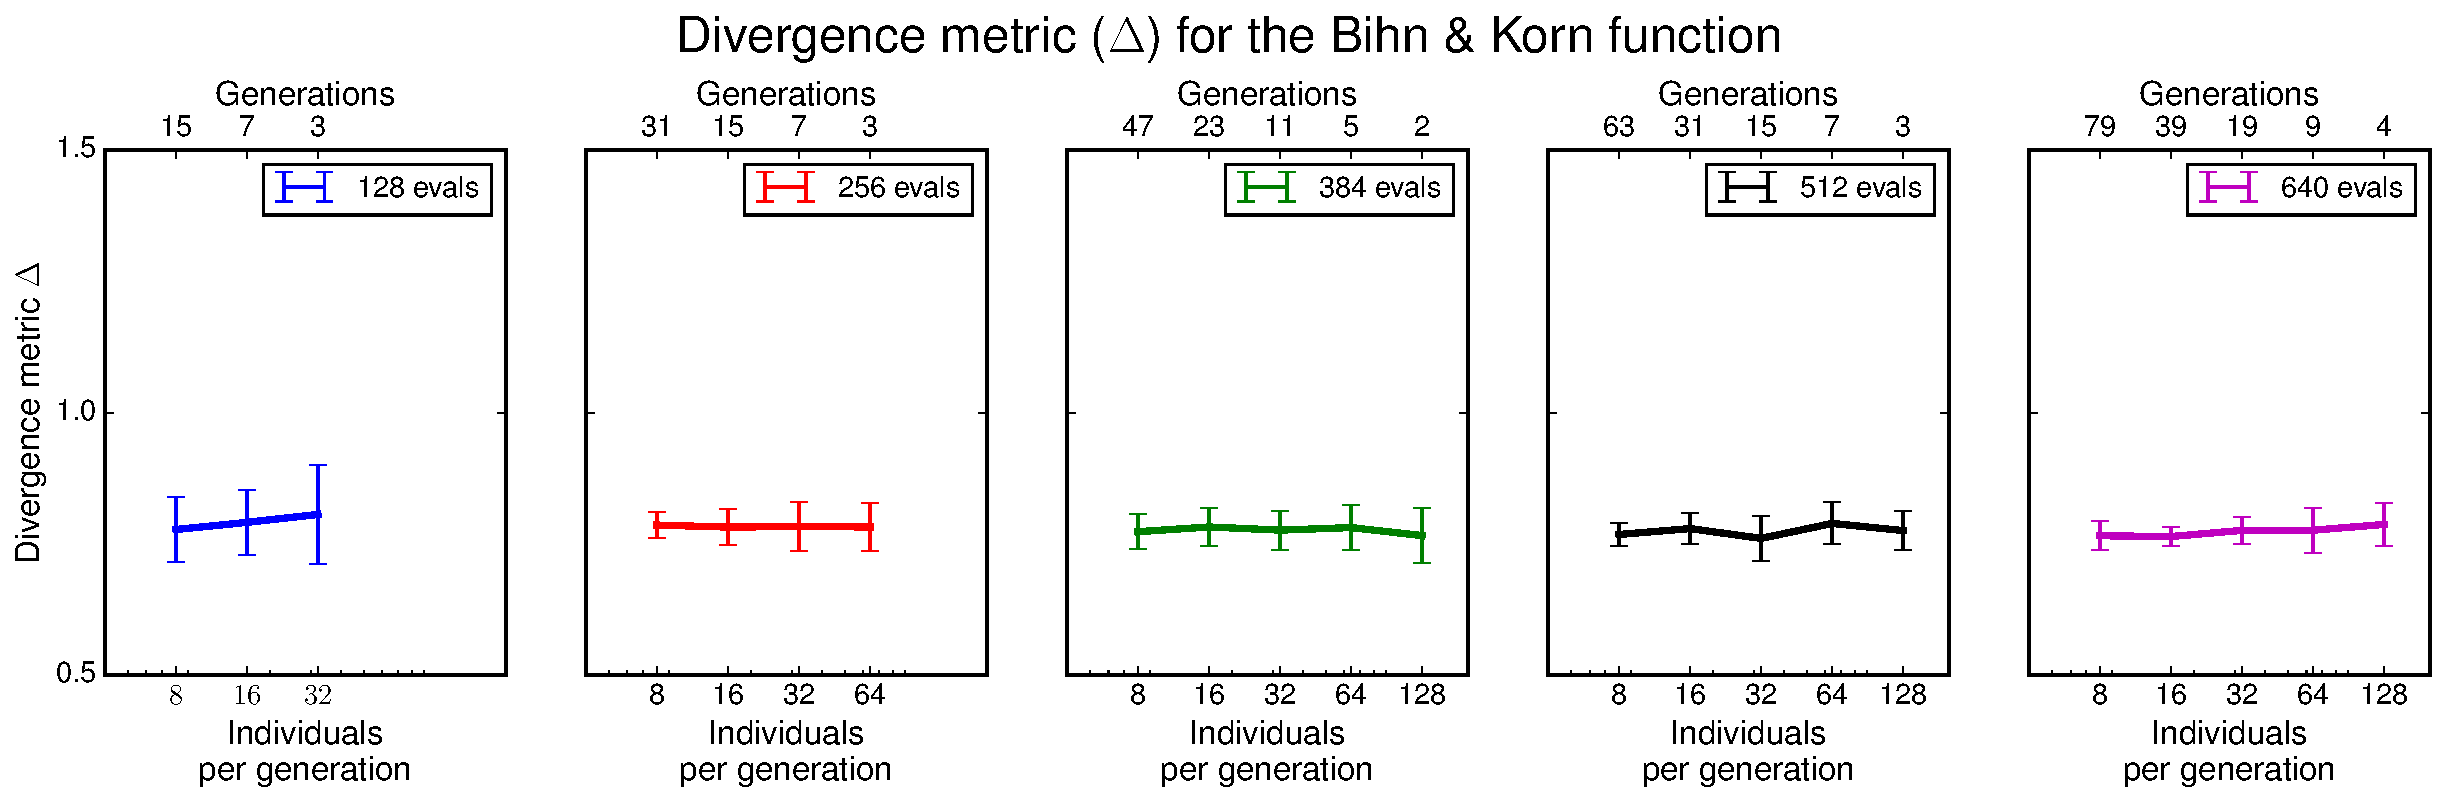
\includegraphics[width=\textwidth]{Figures/3/diverMetric_BK.pdf}
    \end{figure}
    \begin{figure}[h!]
        \centering
        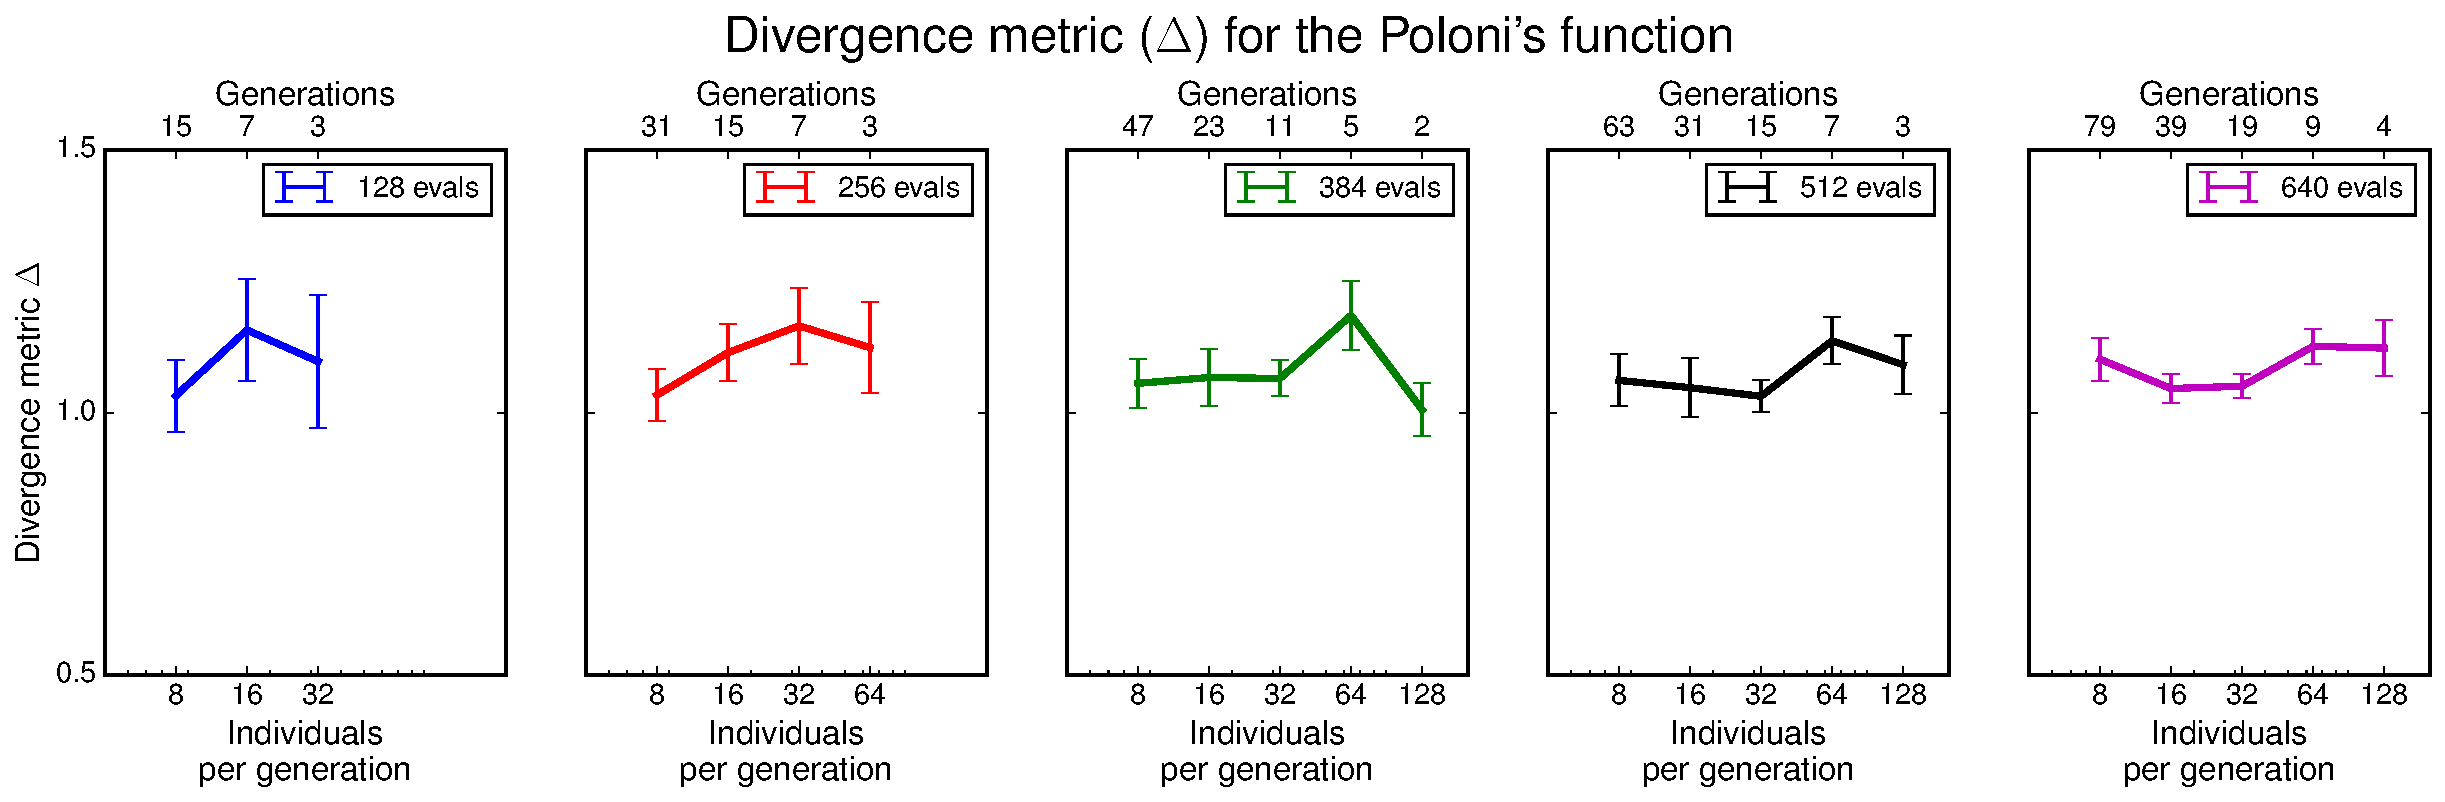
\includegraphics[width=\textwidth]{Figures/3/diverMetric_POL.pdf}
    \end{figure}
    \begin{figure}[h!]
        \centering
        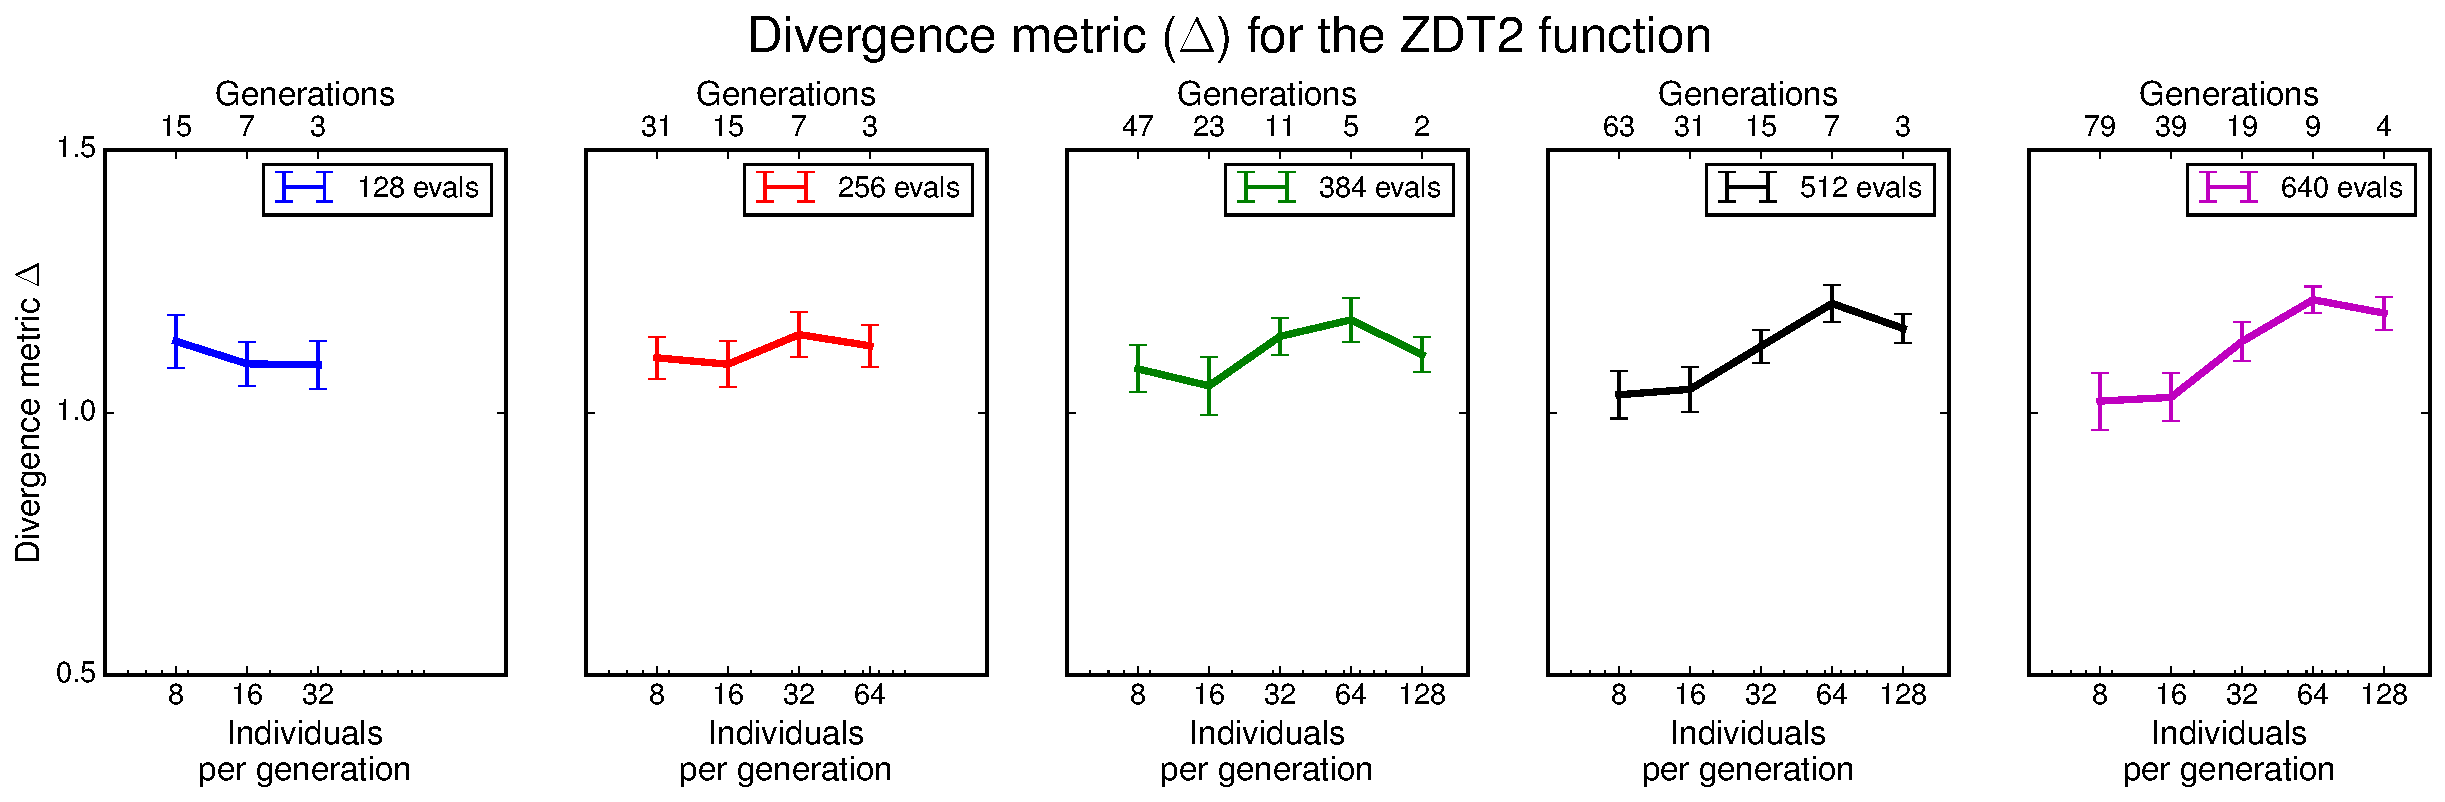
\includegraphics[width=\textwidth]{Figures/3/diverMetric_ZDT.pdf}
        \caption{Divergence metric for the three different test functions}
        \label{fig:diverMetric}
    \end{figure}

The convergence metric ($\Upsilon$) results are shown in Figure \ref{fig:convMetric}. In this case, there is a clear trend: the convergence to the True Pareto front increased with more individuals per generation that with more generations of smaller populations. It must be noted that the first figure in \ref{fig:convMetric} has different vertical limits. However, what is really important is the trend that the metric follow. The results for the ZDT2 function also reveal that the number of generations may be kept small but allowing the population to converge to a solution. Thus, creating a population of very large size and evaluating it just for 3 or 4 generations will not give accurate solutions. 

    \newpage
    
    \begin{figure}[h!]
        \centering
        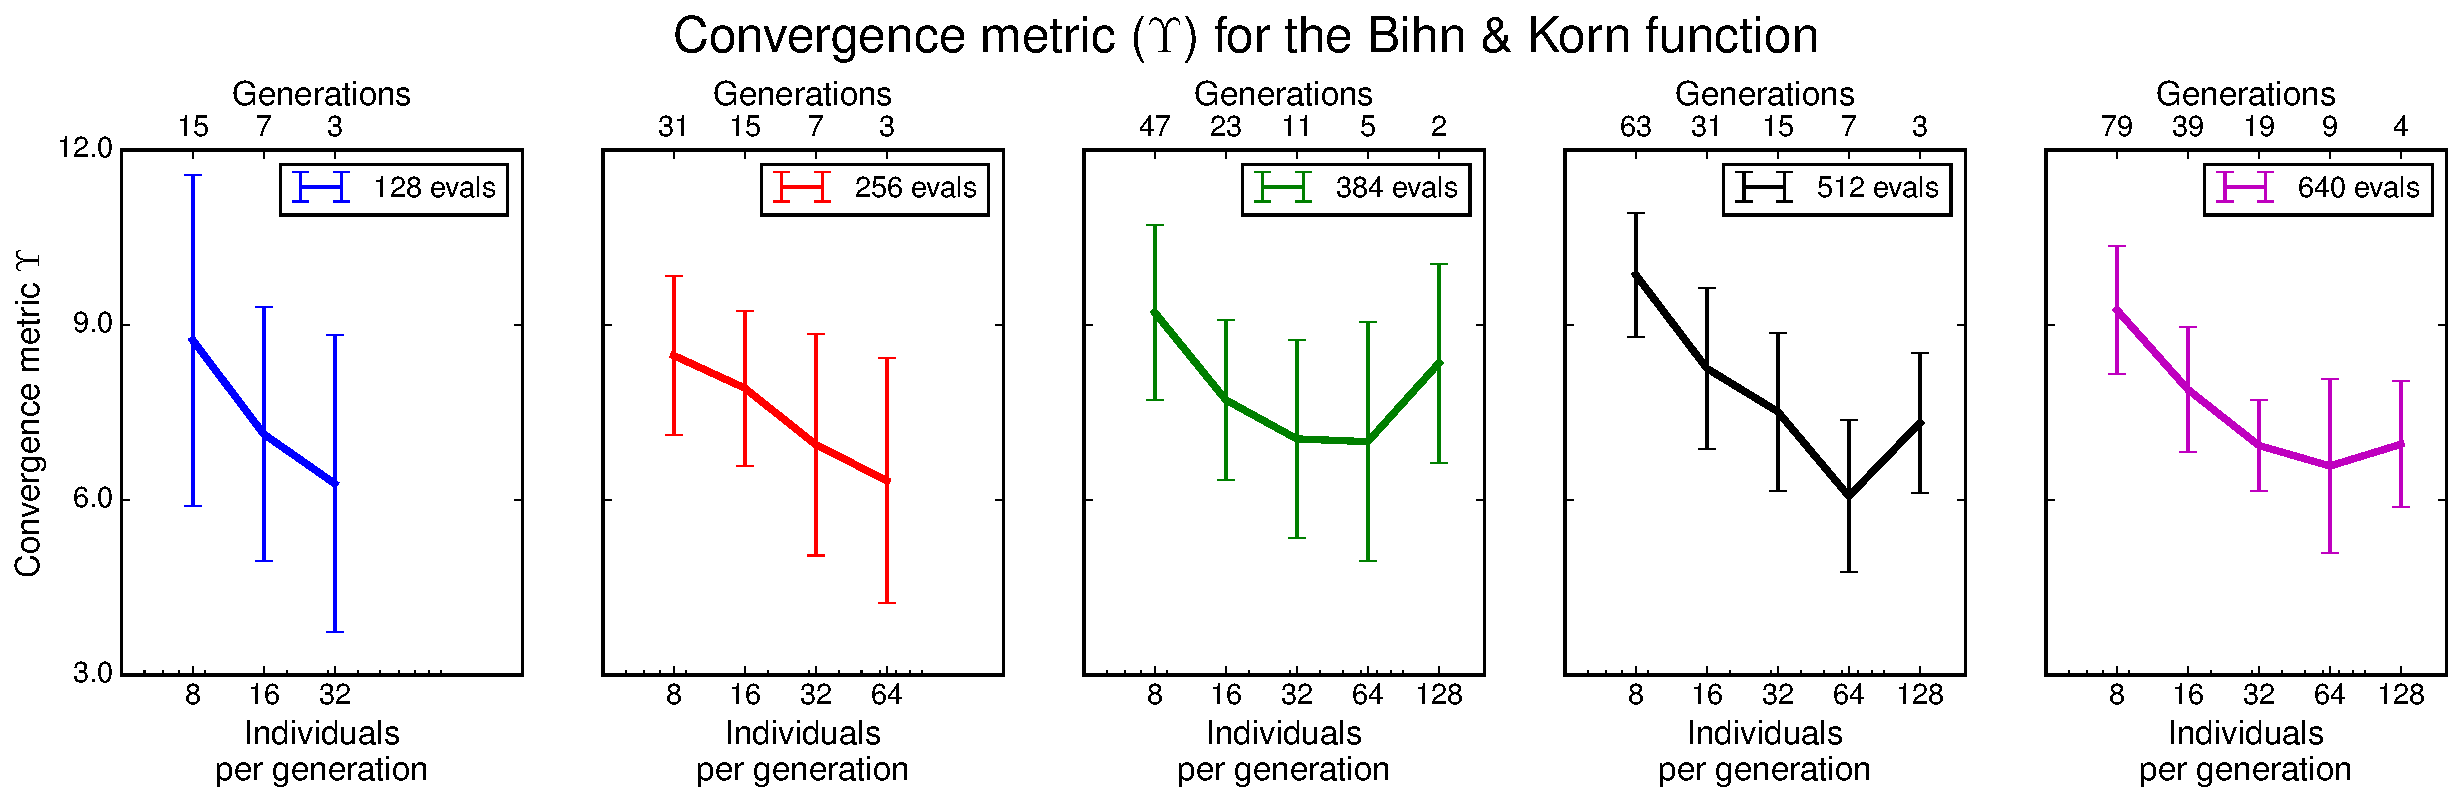
\includegraphics[width=\textwidth]{Figures/3/convMetric_BK.pdf}
    \end{figure}
    \begin{figure}[h!]
        \centering
        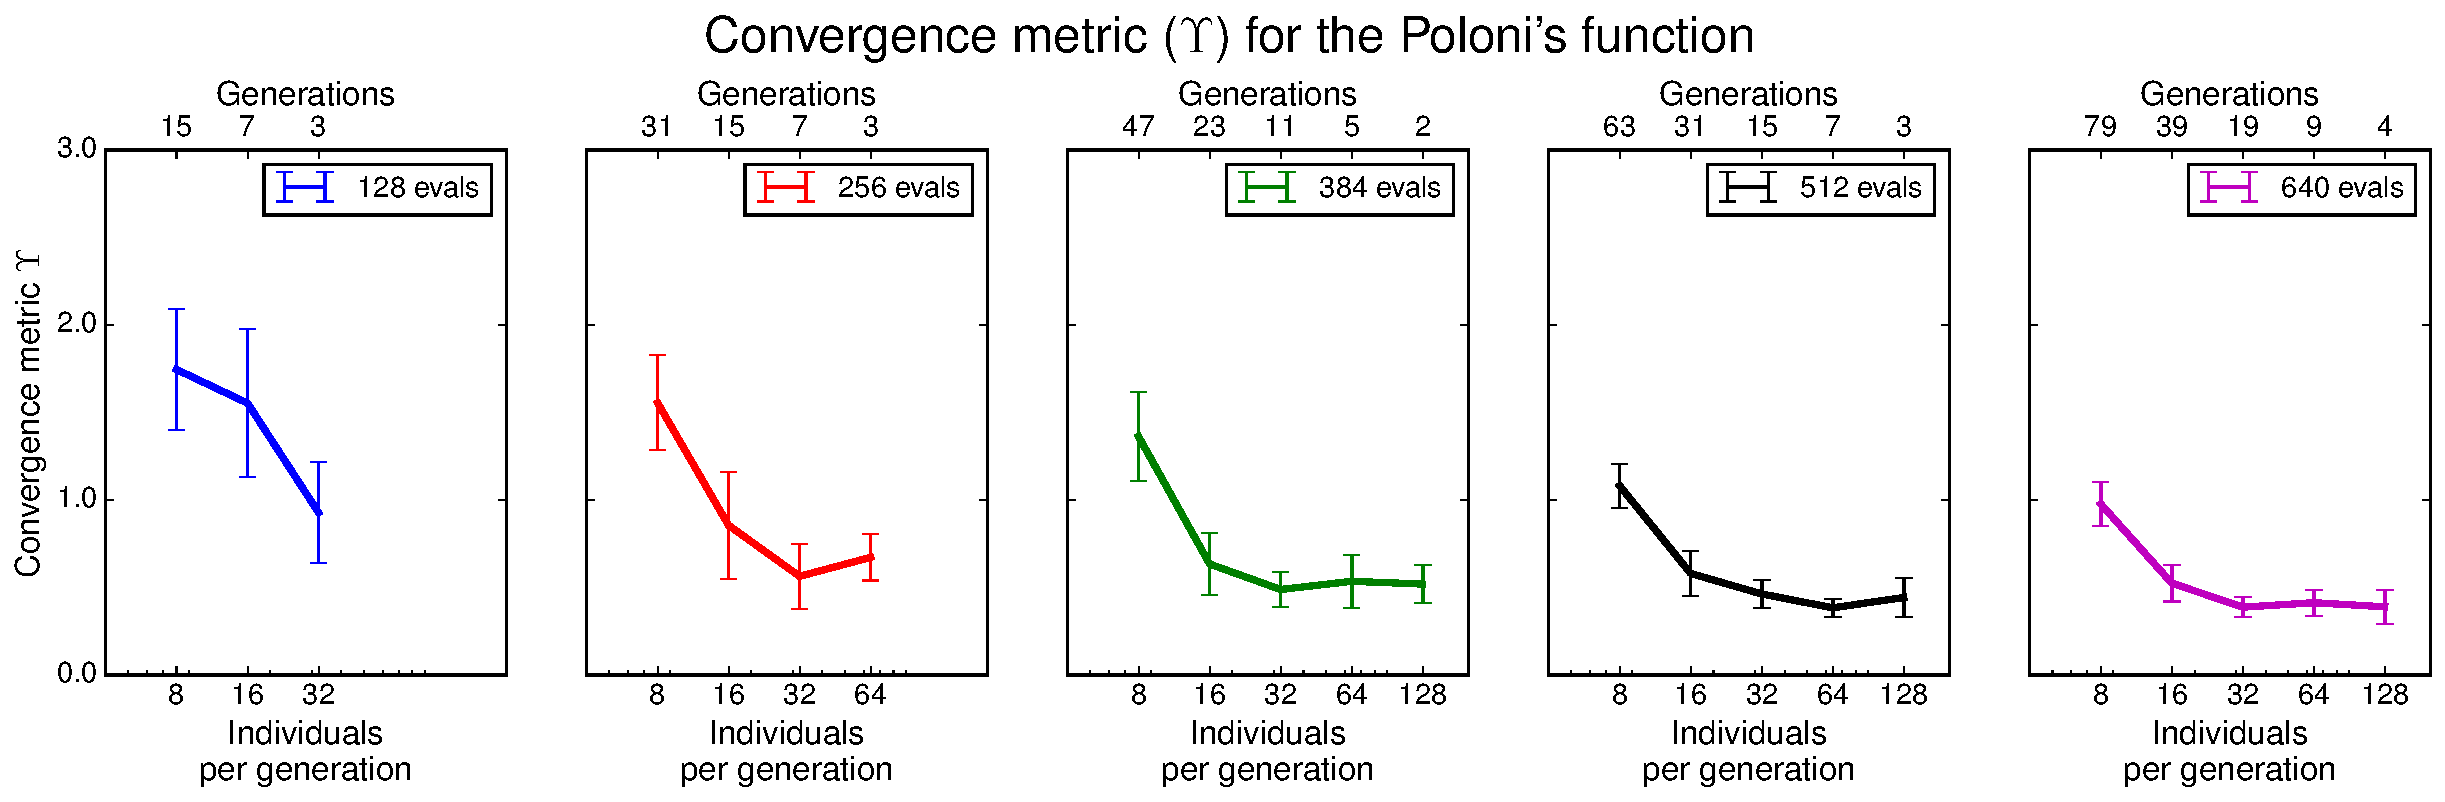
\includegraphics[width=\textwidth]{Figures/3/convMetric_POL.pdf}
    \end{figure}
    \begin{figure}[h!]
        \centering
        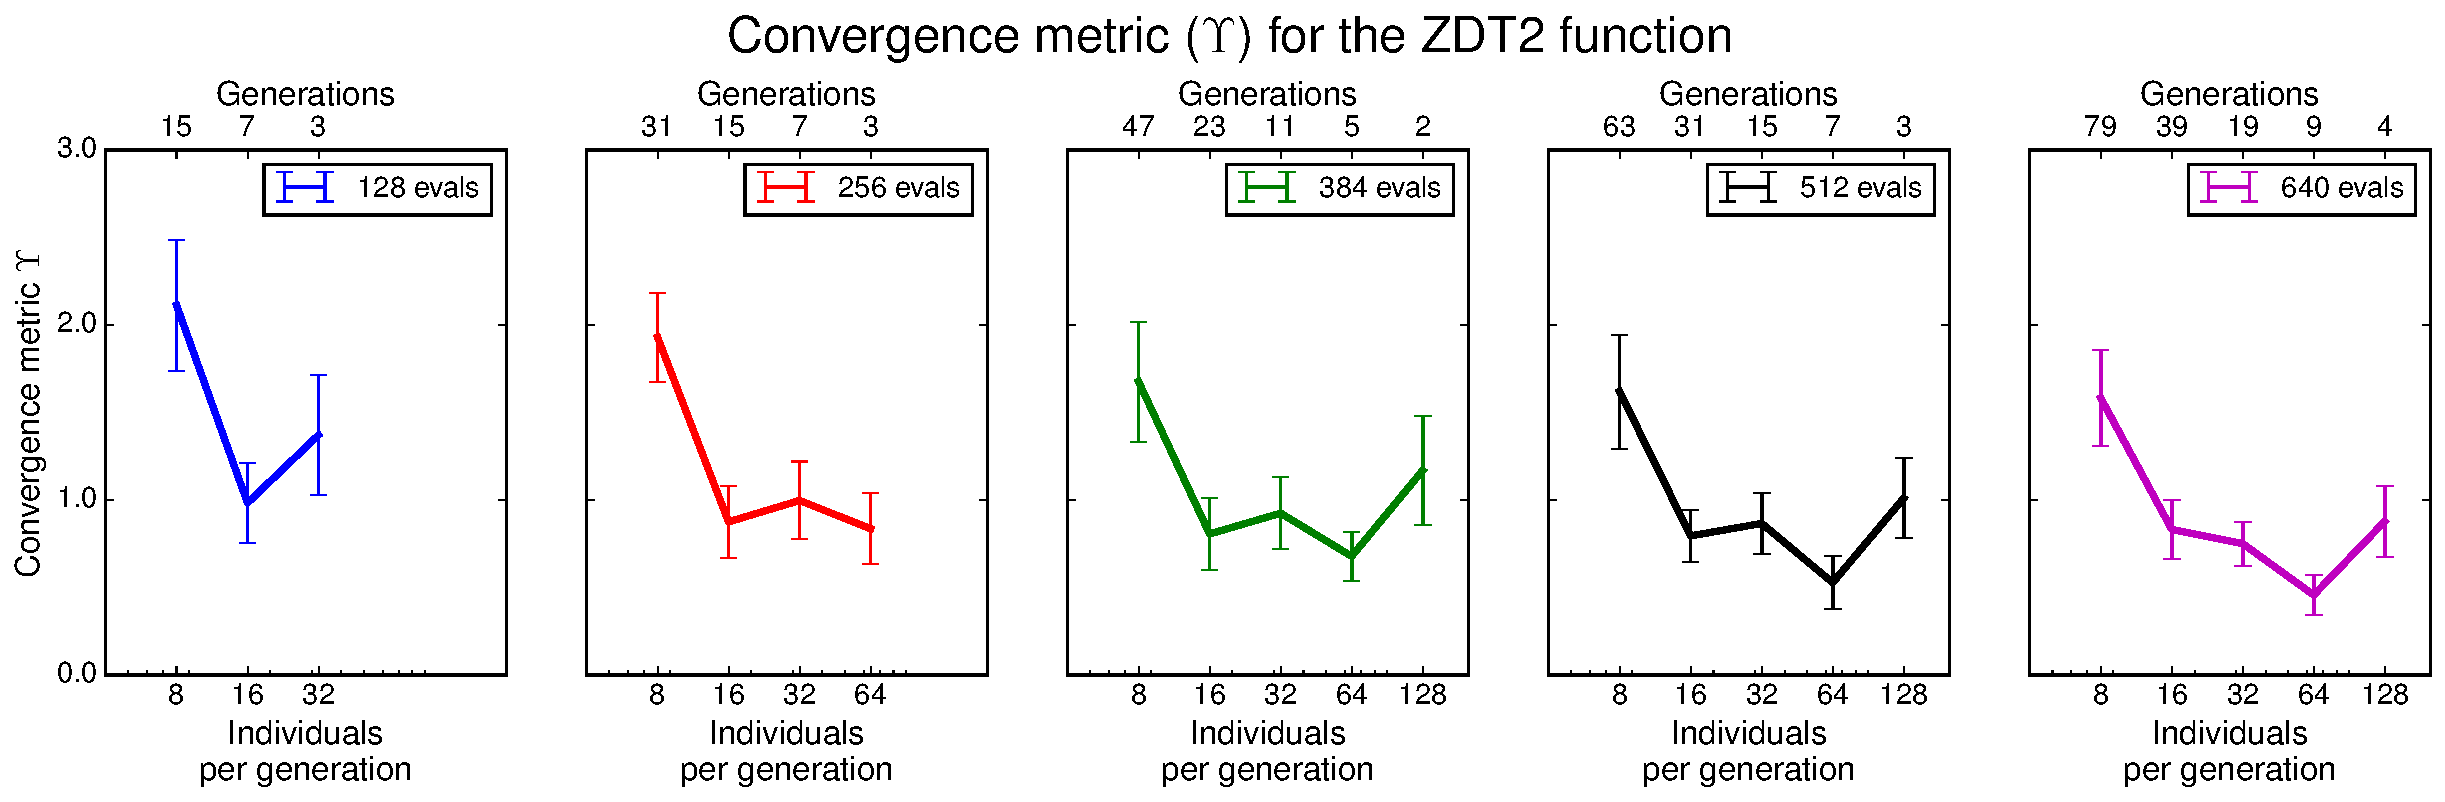
\includegraphics[width=\textwidth]{Figures/3/convMetric_ZDT.pdf}
        \caption{Convergence metric for the three different test functions}
        \label{fig:convMetric}
    \end{figure}
   
\newpage

\section{CFD cases}

In this subsection, different CFD setups will be presented and explained (showing the results in the following section). The code of the NSGA-II was implemented in Python for a two variable and two function case (although it may be easily upgraded to a higher number of variables and objective functions). The different individuals were generated from Python scripts that transformed the variables into a mesh or a configuration file for a case. Each individual has been simulated with OpenFOAM in a parallel fashion (using MPI for multiprocessor parallel computing). The results obtained from the simulation were analyzed with ParaView (in the \texttt{pvbatch} mode) or directly with Python to get the fitness value of each individual. With that fitness value, the genetic algorithm computed the next generation, sending it to OpenFOAM as before. All this loop was controlled with Bash scripting: from running the simulations and waiting for them to finish before sending the next set to calling the different scripts for every individual and generation. Only 2D cases were analyzed, although the procedure for 3D cases will be the same.

The workstation used to perform the different cases was a machine with 32 processors (Intel Xeon CPU E5-2650 @ 2.00GHz), 64 Gb of RAM memory and a 275 Gb SSD hard disk. The machine was running under Ubuntu 16.04 LTS, with OpenFOAM version 5.00, ParaView v5.4.0 and Python 3.6.4. The amount of data obtained after the simulation process almost fill the whole solid state drive, so listing the whole code is unfeasible. However, the basic files for performing the different cases are available in GitHub (\url{https://github.com/jlobatop/GA-CFD-MO}) as well as the code and Jupyter notebooks developed along the process of this thesis. 

\subsection{Suppression of cylinder vortex oscillations}

The first one of the cases is the flow around a cylinder. Although cylinders may seem a very simple case, the results obtained for a cylinder may be extrapolated and used in other cases, such as airfoils. Vortex shedding is a phenomenon that happens when the equilibrium flow around a cylinder suffers a Hopf bifurcation (instability caused by background distances) and the flow enters into a new equilibrium which is time-periodic (at the Strouhal frequency) \cite{sengupta2010dynamical}. This is a major problem when mixing structural behavior and flow dynamics, because if the Strouhal frequency matches the natural frequency of the structure, the consequences may be catastrophic because an excited natural frequency usually leads to unstable behavior of the structure \cite{green2006failure}.

\newpage

There are a lot of ways of suppressing the vortex shed oscillations that are present in the wake of the cylinder. The methods are classified in passive and active, depending if they are looped with some kind of feedback from the state of the system. Vortex shedding may be controlled with a lot of techniques, where the most common ones are magnetic field, rotary oscillations, secondary flow and surface roughness. In this analysis, a passive flow control with a secondary flow will be used. Instead of using a simple blowing jet, a blowing and suction jet will be installed in the rear part of the cylinder. Using a sinusoidal wave that introduces and extracts momentum (instead of a pulse jet that only introduces momentum) avoid issues related to mass conservation in the CFD simulation \cite{rashidi2016vortex}.

\subsubsection*{Case setup}

As said, the flow control will be performed with a sinusoidal wave type of function that depends on two variables: the amplitude ($A$ or $v$ given that the variation in momentum insertion is performed with changes in the velocity) and the frequency ($f$). The initialization of the flow control is performed once the von Karman vortex shedding is already developed, so the phase shift of the sinusoidal wave is fixed. The objective of the optimization is to minimize the force oscillations in both the horizontal and vertical axis. In order to quantify the oscillations, different approaches were considered. The output of the OpenFOAM solver returns a force-time data file that contains the forces that the cylinder is suffering. In order to capture the amplitude of the data obtained, a Fourier transform was at first considered. The amplitude values are very small so the \texttt{FFT} (Fast Fourier Transform) implemented in Python did not work properly. Computing the root mean square (RMS) error was also viewed as a possible approach. The RMS for a data set is defined as \cite{bissell1992digital}:

\begin{equation}
    x_{rms}=\sqrt{\dfrac{1}{n}\left( x_1^2 + x_2^2 + ... + x_n^2 \right)}
\end{equation}

\begin{equation}
    x_{rms}^2=\overline{x}^2+\sigma_x^2=\overline{x^2}
\end{equation} 
where $\bar{x}$ is the mean and $\sigma_x$ is the standard deviation. The problem that this metric has is that it cannot go to zero because the mean $\overline{x}$ will not go to zero given that there is only one exit in the rear part and the force exerted is not compensated with a front membrane (having that $\overline{x}\neq 0$). Thus, scenarios with small forces and large oscillations will have the same RMS value of larger forces but zero oscillations cases. 

The metric that better represent the problem is the standard deviation $\sigma$. Computing it in the last $n$ cycles (where $n$ depends on the complete cycles that have been captured in the simulation), an oscillatory force will only have $\sigma=0$ if the amplitude of the oscillations is zero. Thus, the algorithm will try to minimize $\sigma_Y$ and $\sigma_X$ for a sum of the pressure and viscous forces.

The genetic algorithm setup was done with 64 individuals in the first generation and just 10 individuals for each other generation. A 6 generation limit was also established. These limits may be very strict but they are chosen for computational resources limitations. A more powerful study may be performed, surely achieving more accurate solutions. The search domain is $A\in[0.01,2]$ and $f\in[0.01,\pi/2]$. The solver used is \texttt{pimpleFoam}, which is an incompressible solver for transient cases. The maximum time of simulation was 150 seconds. Newtonian transport model with laminar turbulence modeling was chosen. The case was done in a non-dimensionalized fashion, with a density value of $\rho=1 kg\cdot m^{-3}$, a viscosity value of $\nu=1\times 10^{-5} m^2\cdot s^{-1}$, and a cylinder diameter of $1\ m$ facing a flow at a velocity of $1\ m\cdot s^{-1}$. This values give a Reynolds number of $Re = 100,000$. Vortex shedding at this Reynolds number happens to occur in a turbulent way. Most of the schemes were chosen as \texttt{linear} and the time differentiation scheme was chosen to be \texttt{backward}. The real mesh can be seen in Figure \ref{fig:cylMeshSChematicsPF} and the mesh details are shown in Figure \ref{fig:cylMeshSChematics}.


    \begin{figure}[h!]
        \centering
        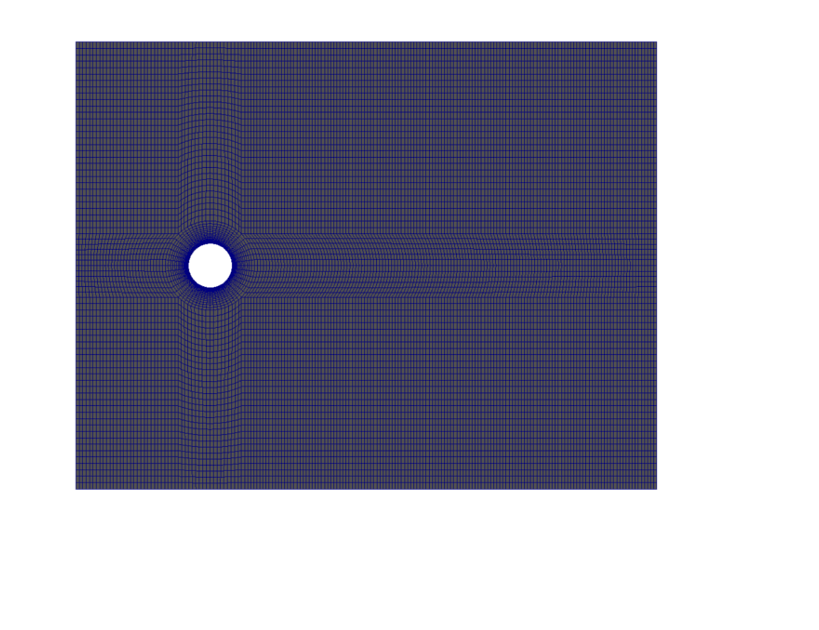
\includegraphics[width=0.8\textwidth]{Figures/3/cylinderMeshPF.png}
        \caption{Picture of the mesh for the cylinder case}
        \label{fig:cylMeshSChematicsPF}
    \end{figure}

\newpage

    \begin{figure}[h!]
        \centering
        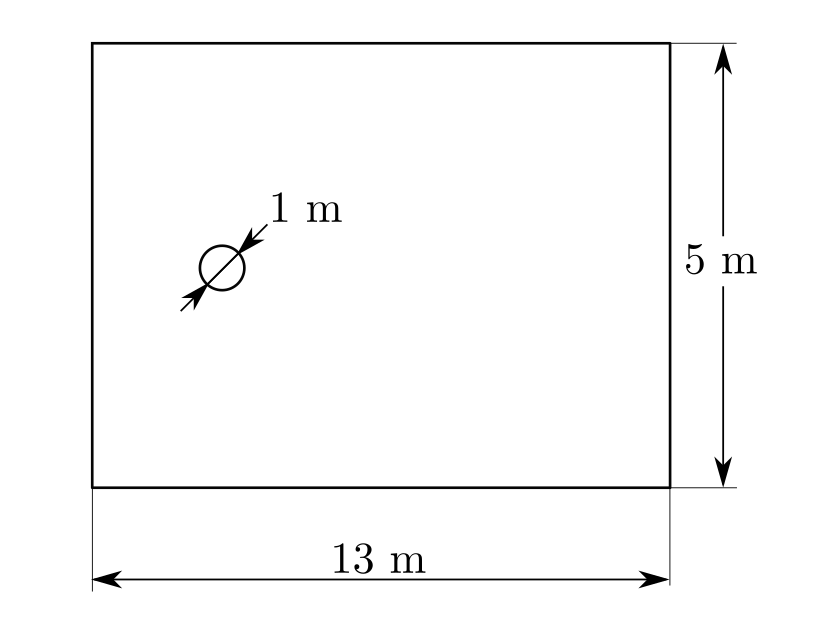
\includegraphics[width=0.6\textwidth]{Figures/3/cylinderMesh.png}
        \caption{Schematics of the mesh for the cylinder analysis}
        \label{fig:cylMeshSChematics}
    \end{figure}


The boundary conditions imposed in the different faces are listed with an exploded view of the mesh. 

  
      \begin{table}[h!]
        \centering
        \caption{Boundary conditions for the cylinder case}
        \label{fig:tableCylBC}
        \begin{tabular}{cc}
        \multicolumn{2}{c}{\textbf{Inlet (yellow)}}          \\
        \hline
        $U$                    & \texttt{fixedValue (1 0 0)}           \\
        $p$                     &  \texttt{zeroGradient}          \\
        & \\
        \multicolumn{2}{c}{\textbf{Outlet (green)}}          \\
        \hline
        $U$                    & \texttt{zeroGradient}           \\
        $p$                     &  \texttt{fixedValue 0}          \\
        & \\
        \multicolumn{2}{c}{\textbf{Flow control membrane (grey)}}      \\
        \hline
        $U$                    & \begin{tabular}{c}
             \texttt{uniformFixedValue} \\
             \texttt{(tableFile)}
        \end{tabular}           \\
        $p$                     &  \texttt{zeroGradient}          \\
        & \\
        \multicolumn{2}{c}{\textbf{Upper/Lower (grey)}}      \\
        \hline
        $U$                    & \texttt{symmetry}           \\
        $p$                     &  \texttt{symmetry}          \\
        & \\
        \multicolumn{2}{c}{\textbf{Cylinder (red)}}      \\
        \hline
        $U$                    & \texttt{fixedValue (0 0 0)}           \\
        $p$                     &  \texttt{zeroGradient}          \\
        & \\
        \multicolumn{2}{c}{\textbf{Front/Back (white)}}      \\
        \hline
        $\texttt{*}$                    & empty \\
        \end{tabular}
        \end{table}

\newpage

     \begin{figure}[h!]
        \centering
        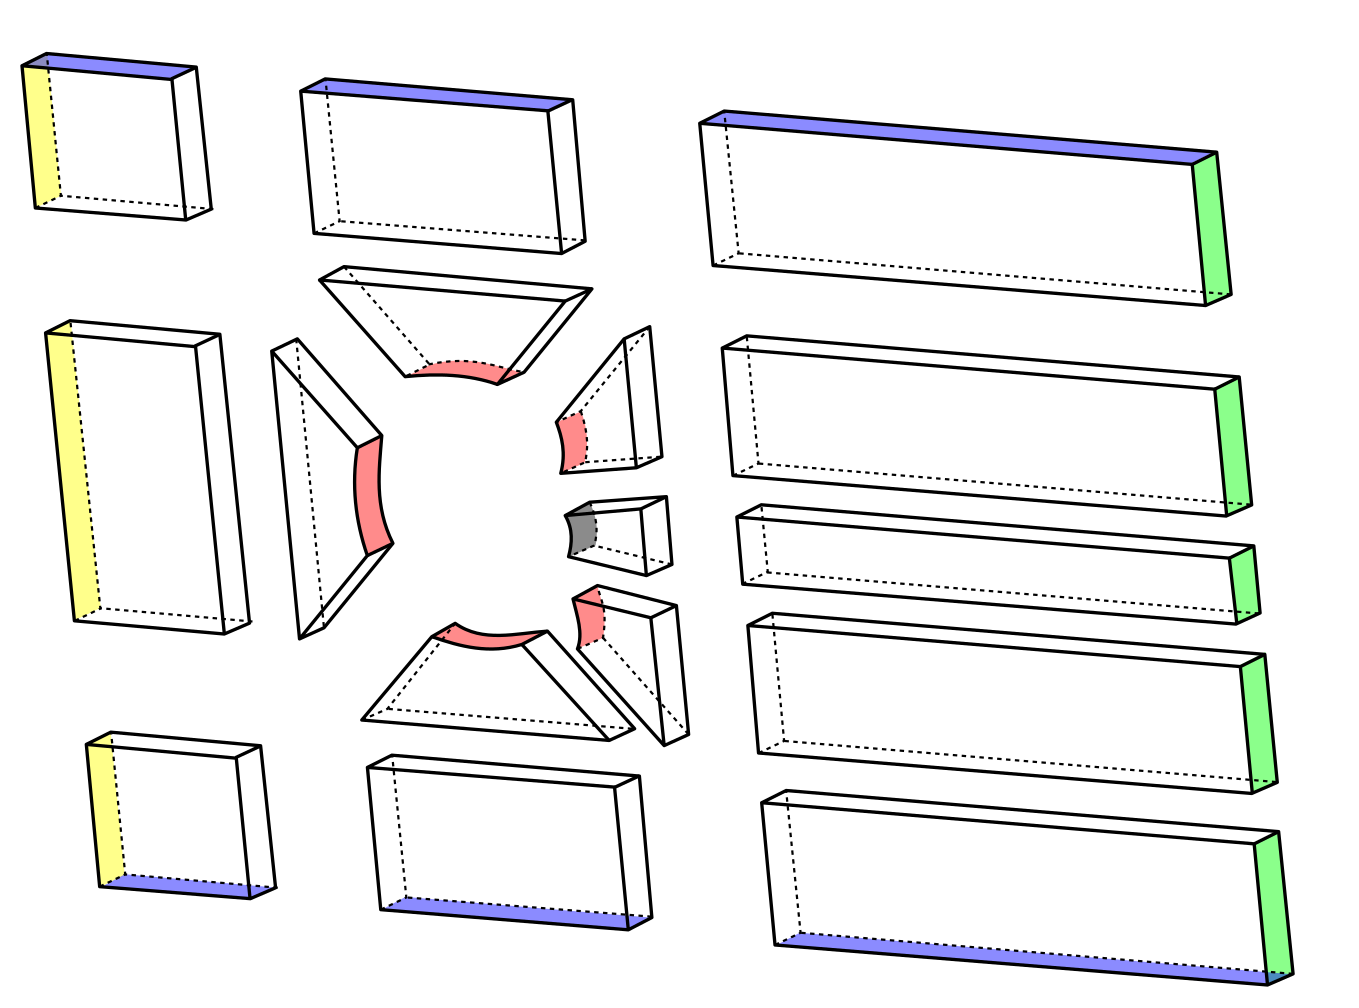
\includegraphics[width=0.55\textwidth]{Figures/3/cylinderMeshBC.png}
        \caption{Exploded view of the mesh for the cylinder case}
        \label{fig:cylBC}
    \end{figure}


\subsection*{Processor convergence}

Apart from the typical mesh convergence studies, the processor convergence type of analysis is critical in this highly parallelizable cases. One simulation may be divided for a different number of processors, having that time reaches a minimum in some number of processors. Total simulation time is the sum of the simulation time, case decomposition time and case reconstruction time. For 1 processor there are no decomposition nor reconstruction times, so the total time is the same as the simulation time. 

     \begin{figure}[h!]
        \centering
        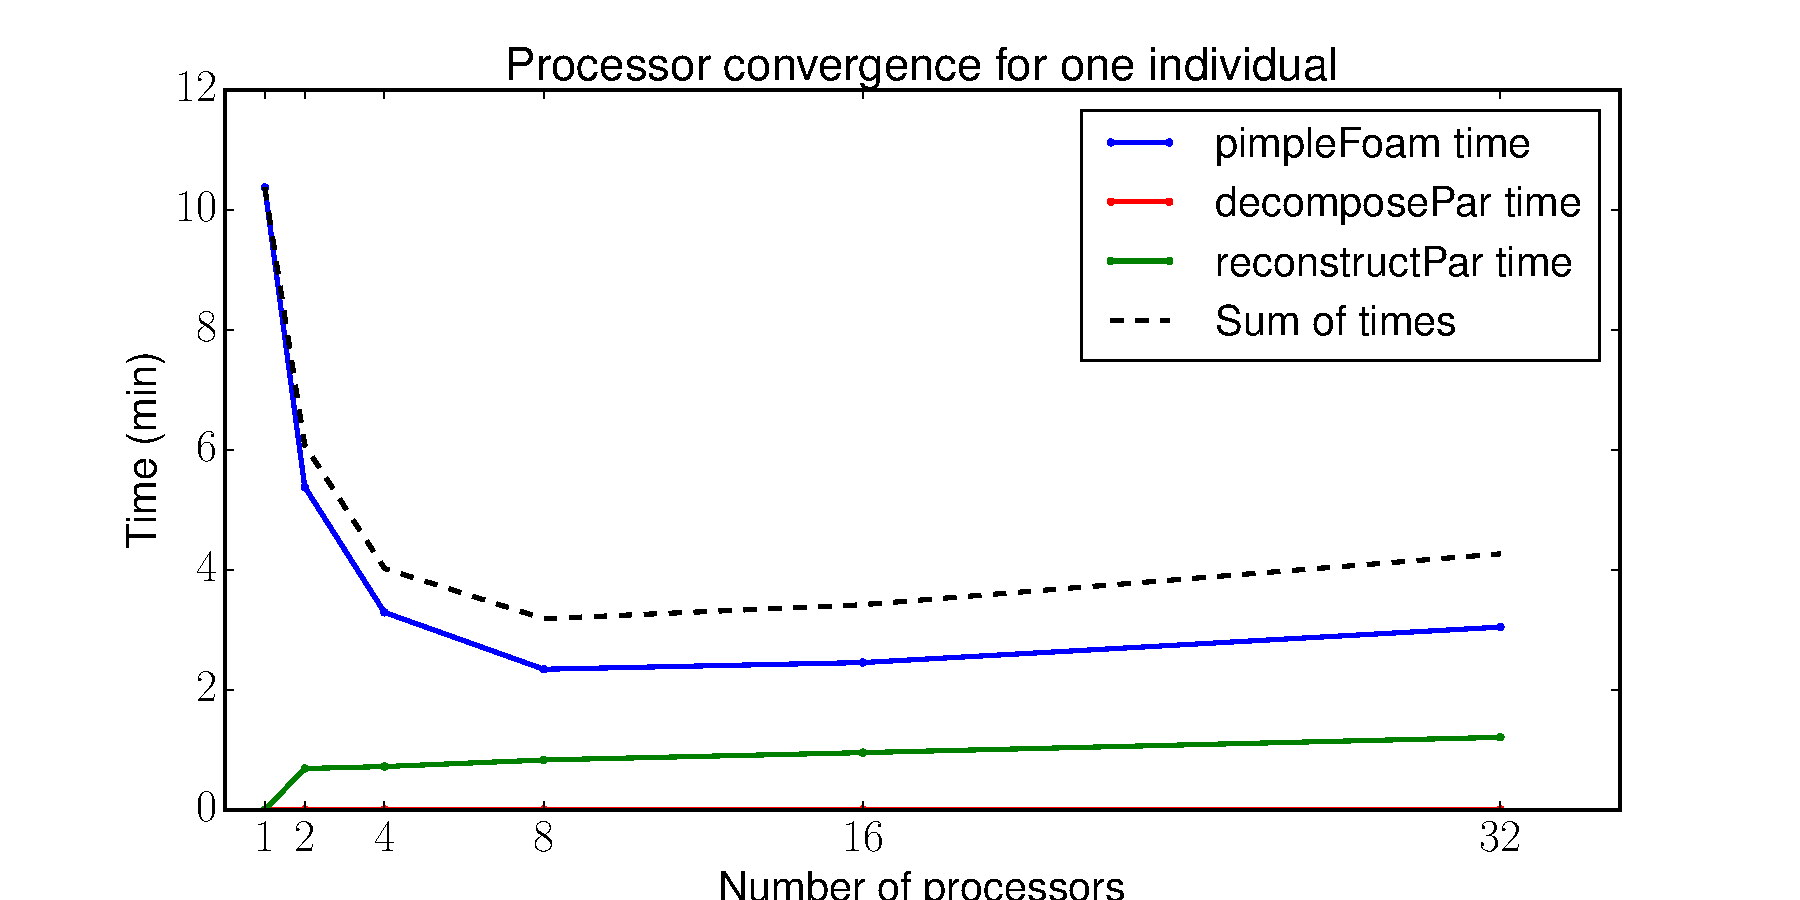
\includegraphics[height=0.35\textheight]{Figures/3/procConv_1ind.pdf}
        \caption{Processor convergence for 1 individual}
        \label{fig:procConvergenceCyl}
    \end{figure}

\newpage

The results of the processor convergence in Figure \ref{fig:procConvergenceCyl} shown that using $8$ processor gives the fastest results. However, when applying genetic algorithms or another population-based algorithm, there are a lot of simulations that might be performed at the same time. If each individual is computed in 1 processor (and constraining the problem to a 32-processors machine), then 32 individuals may be computed at the same time. If each individual is simulated in 2 processors, only 16 individuals may be run at the same time (so if each population is formed by 32 individuals, 16 must be simulated first and 16 once the latter have finished). If each individual is run in 4 processors, only 8 individuals may be simulated at the same time, sending the population into 4 groups of 8. 


If the sum of times from one individual is multiplied by the divisions that must be made to a generation of $32$ individuals for simulating the whole population, an estimation of the simulation time is obtained. Nevertheless, the real times were computed and plotted in Figure \ref{fig:genProcConvergenceCyl}, seeing that there is a difference between the actual values and the estimated ones (probably due to the fact that there are computational resources that were not affected in the one individual simulation times).  

     \begin{figure}[h!]
        \centering
        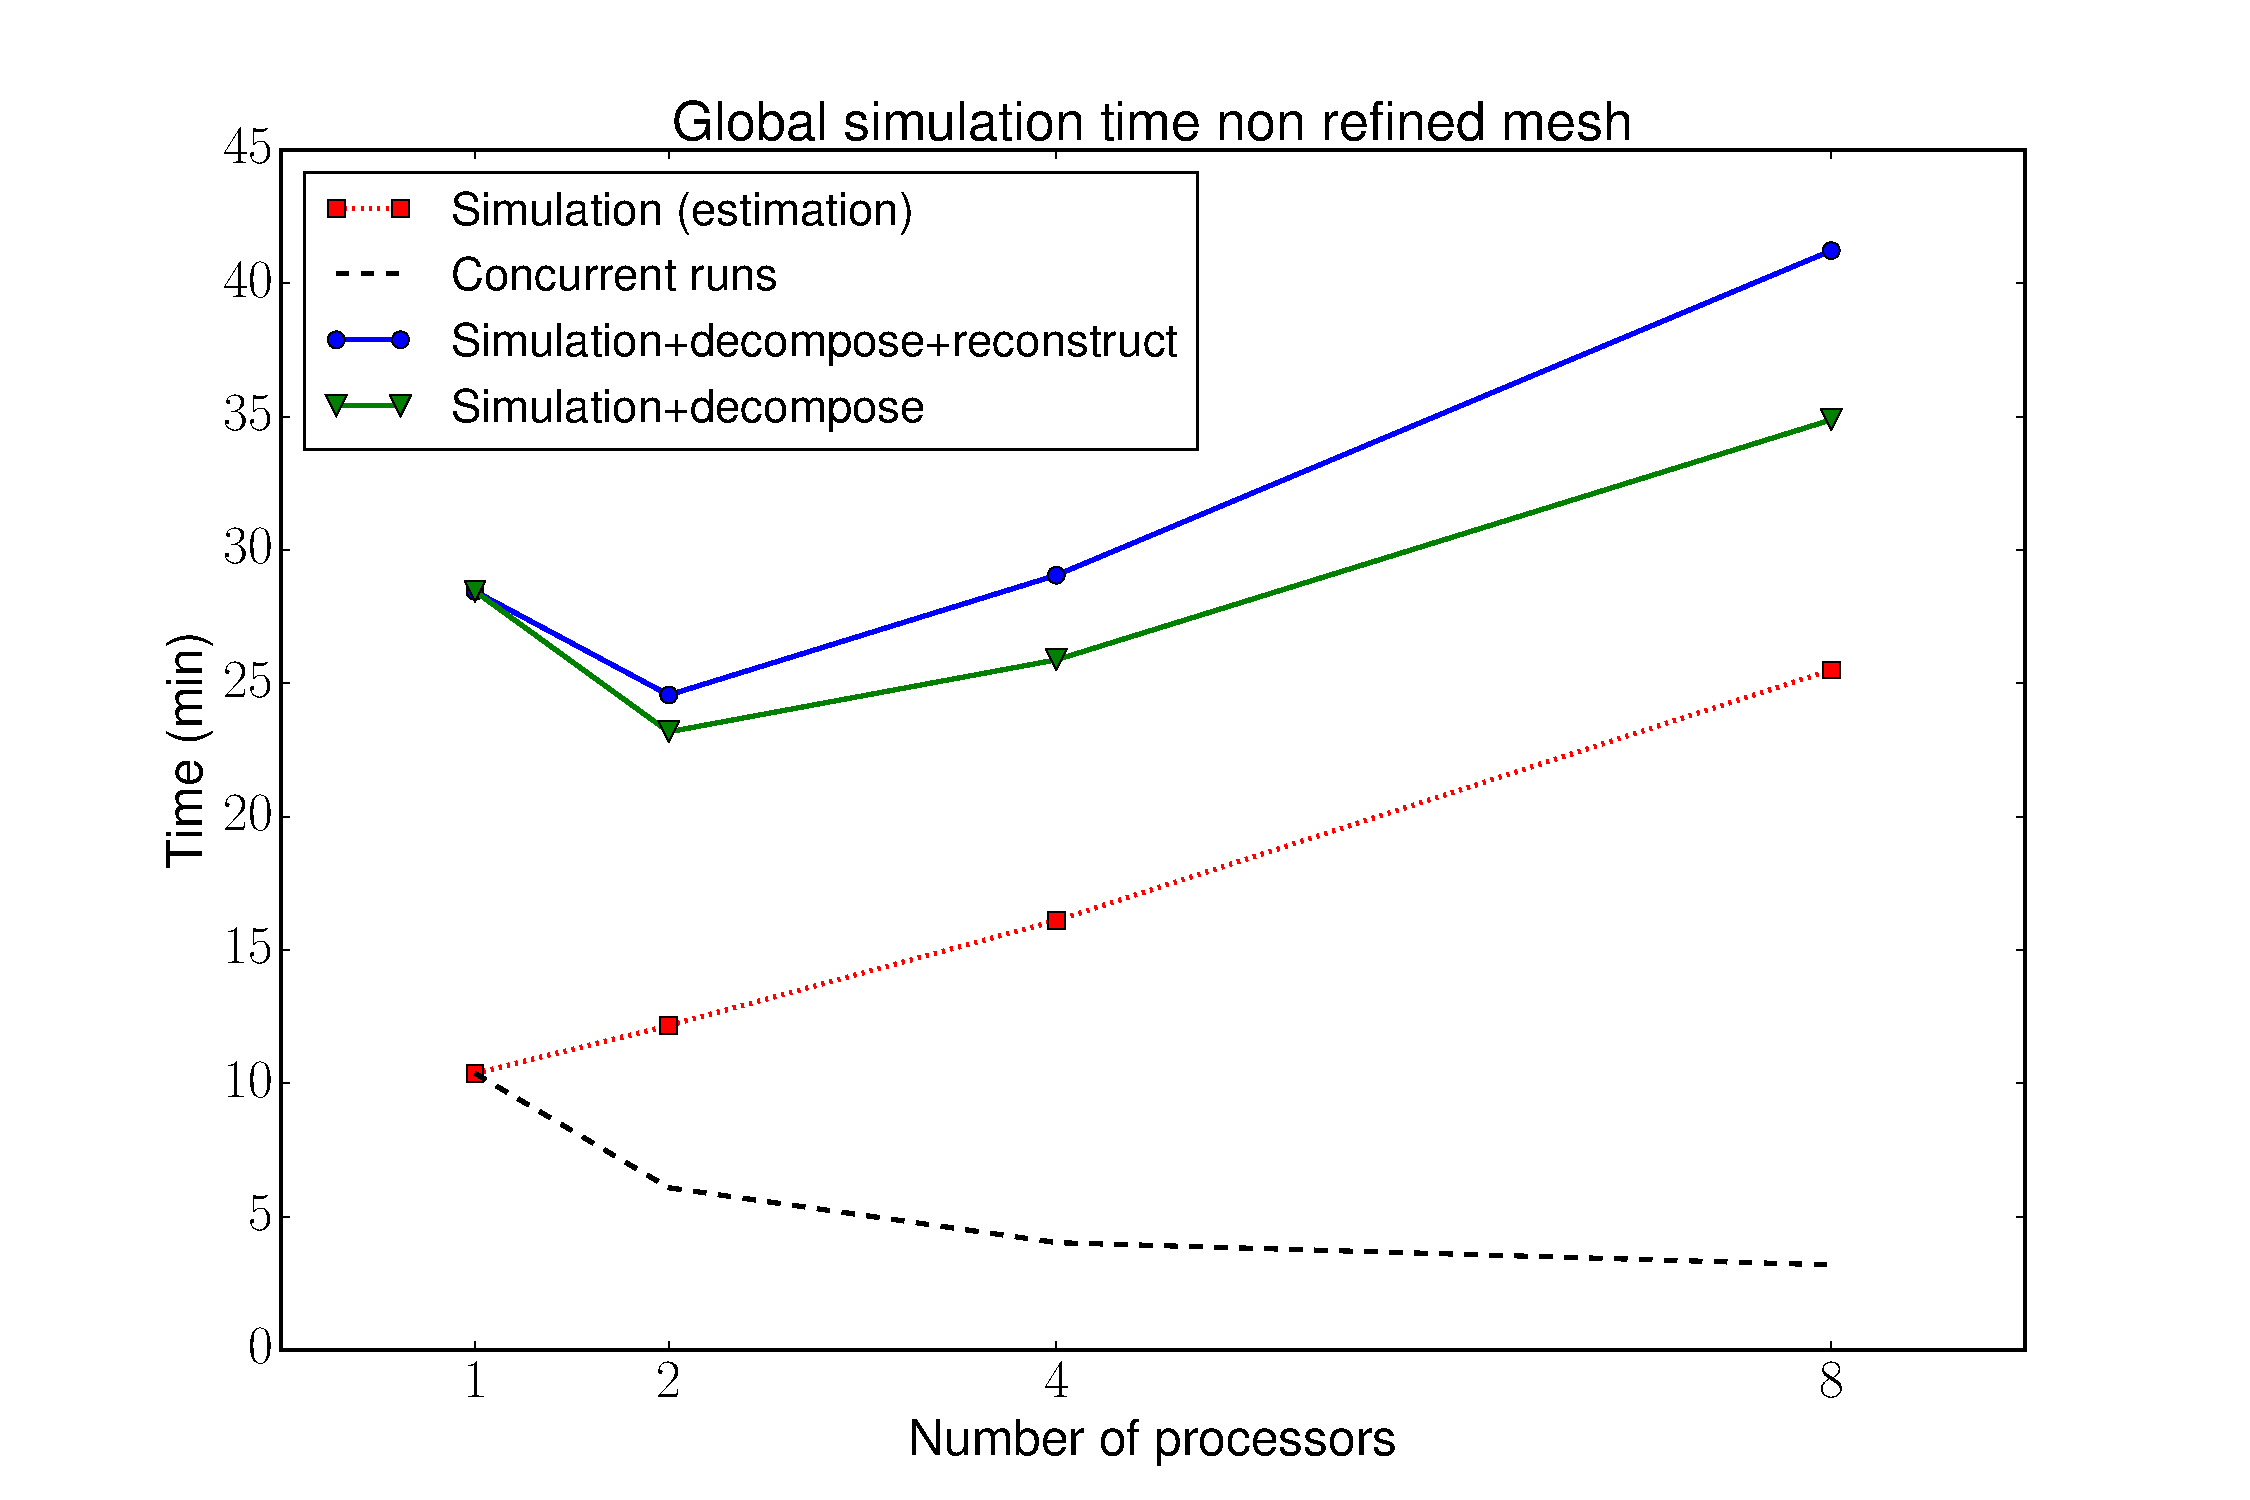
\includegraphics[width=0.85\textwidth]{Figures/3/procConv_1gen2.pdf}
        \caption{Processor convergence for a 32 individual population}
        \label{fig:genProcConvergenceCyl}
    \end{figure}

The reconstructed time has been separated from the decomposition time because in order to analyze the results it is not strictly necessary to reconstruct the case. This does not make any difference because, for all the cases, the most optimal configuration is to use 2 processors. 

\newpage

\subsection{Inlet of diffuser geometry}

Optimizing the inlet of a diffuser is the first step for increasing the efficiency and performance of the engine as a whole. Inlet diffuser geometry is a well-known problem that has been studied in multiple approaches \cite{djebedjian2004two}, \cite{schmandt2011diffuser}. However, there are a lot of shapes in which the inlet may be optimized, e.g., if multiple variables are analyzed, the shape may be parametrized with splines or with control nodes. For simplification purposes, in this study the shape was computed with two values: a length ($L$) and an angle ($\theta$), which are the search space variables. The function space is formed by the total pressure ratio (computed between the total pressure in the outlet of the diffuser and the freestream total pressure) and by the Mach number in the diffuser outlet. Both values will be maximized. The first one seems evident to maximize: total pressure ratio is related to entropy generation and the lower the entropy generation, the better. The maximization of the Mach number in the outlet of the diffuser may be useful in supersonic combustion engines, where there is not turbomachinery and the flow may enter at supersonic speeds to the diffuser \cite{cain2002review}. 

\subsubsection*{Case setup}

In this case, instead of varying the flow conditions as before, the optimization will be performed to the mesh. Thus, each combination of $L$ and $\theta$ will have an associated mesh, having all the meshes with the same boundary conditions of $M_\infty$, $p_\infty$ and $T_\infty$. A combination of the two may be performed, having, for example, $L$ and $Ma$ as the search space variables to maximize both the pressure ratio and the Mach number at the diffuser outlet (having the problem of the moving inlet of the SR-71 Blackbird).  Both the Mach number and the total pressure ratio are computed in Python with values extracted from Paraview. The genetic algorithm used 32 individuals per generation and 6 generations limit. This simulation was performed with a compressible steady state solver (\texttt{rhoSimpleFoam}) with 2500 maximum iterations, where the residuals were stable. The turbulence modeling was done with a $k-\epsilon$ model under Newtonian fluid and perfect gas assumptions. The freestream velocity was $u_\infty = 590\ m\cdot s^{-1}$ which for a temperature of $T_\infty=216\ K$ yields a Mach number of $Ma=2$, freestream pressure was $P_\infty=19930\ Pa$ which corresponds to a altitude of $12\ km$, viscosity was $\nu=1\times 10^{-5} m^2 \cdot s^{-1}$ and the density $\rho=0.31\ kg \cdot m^{-3}$. $k$, $\epsilon$, $\nu_t$ and $\alpha_t$ were chosen based on the tutorials in the OpenFOAM library. The Reynolds number for this case will vary depending on both the horizontal length $L$ and the inclination angle $\theta$, but it will be located near the $Re \sim 10^6-10^7$ range.

\newpage

The geometry of the mesh is sketched in Figure \ref{fig:diffuserMesh}, having some fixed distances for all possible individuals and some variable dimensions: $L$ and $\theta$. Fixed distances will constrain the possible dimensions that the step may have and they are necessary to avoid having a completely undefined problem. Python took each combination of $L$ and $\theta$, created a \texttt{blockMeshDict} with the corresponding dimensions and then run the file to get the mesh. 

     \begin{figure}[h!]
        \centering
        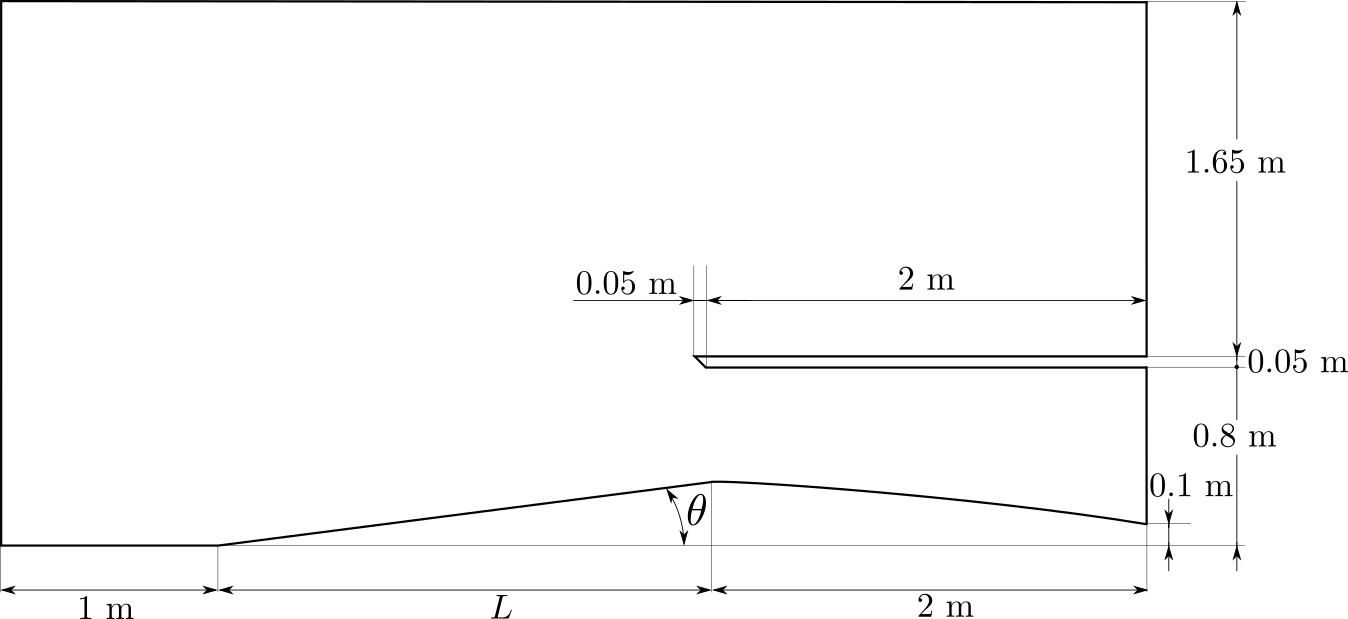
\includegraphics[width=0.85\textwidth]{Figures/3/diffuserMesh.png}
        \caption{Schematics of the mesh for the diffuser mesh}
        \label{fig:diffuserMesh}
    \end{figure}

One possible set of values $L-\theta$ returned the mesh shown in Figure \ref{fig:diffuserMeshPF}. It can be seen that the grading of the mesh is concentred in some zones while other zones have a more coarse grid. Given that \texttt{blockMesh} uses hexahedral blocks, the refinement must be performed along the dimensions of the hexahedral. This is a 2D case so in the spanwise direction $z$ there is only one cell (not shown in the picture).

     \begin{figure}[h!]
        \centering
        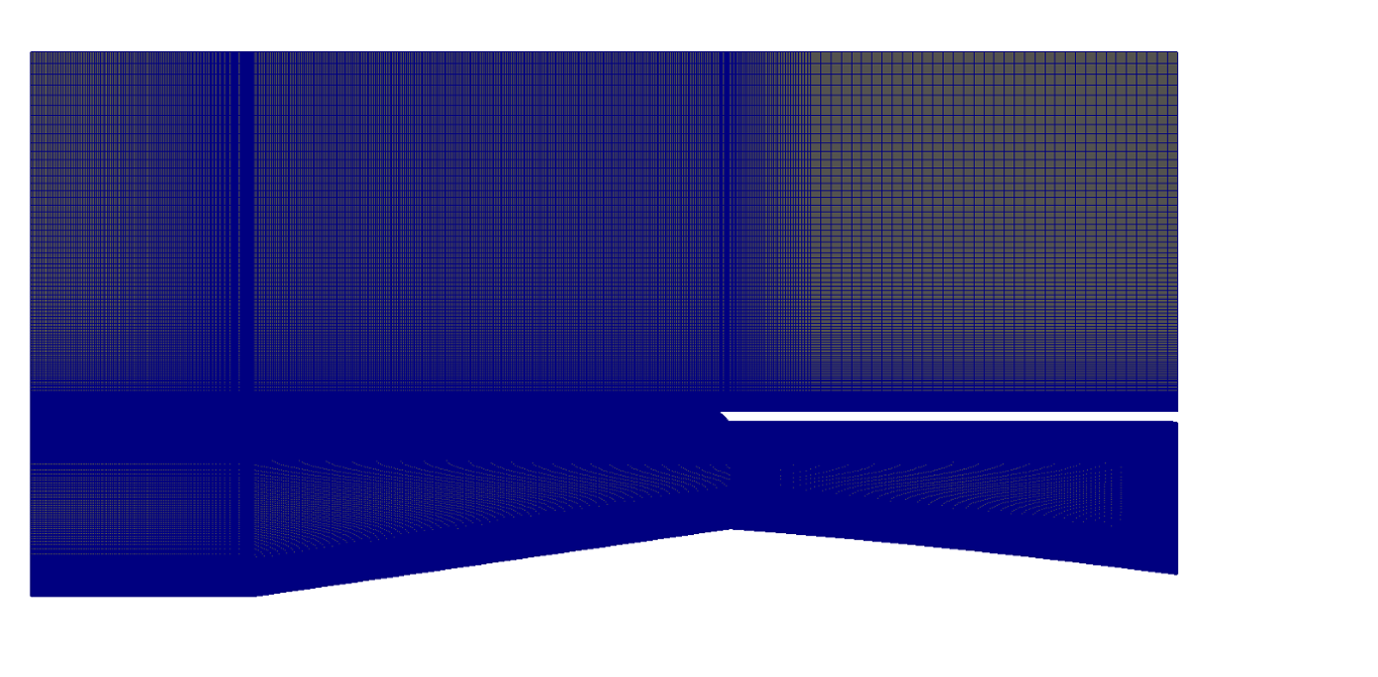
\includegraphics[width=0.86\textwidth]{Figures/3/diffuserMeshPF.png}
        \caption{Picture of the mesh for diffuser case (random $L$ and $\theta$)}
        \label{fig:diffuserMeshPF}
    \end{figure}
    
   \newpage
   
   As it has already been mentioned, the fixed dimensions of the mesh will bound the possible values that $L$ and $\theta$ take. The heights of $0.1\ m$ and $0.8\ m$ inside the diffuser will constraint the maximum and the minimum value of $\theta$ for each $L$. There is also $\theta^{phys}_{max}$ given by the attached oblique shock wave theory. It will only depend on the value of $M_\infty$, having a maximum angle limitation independent of the length $L$. Finally, a maximum length $L_{max}$ was fixed in order to avoid unrealistic lengths of the step.
      
     \begin{figure}[h!]
        \centering
        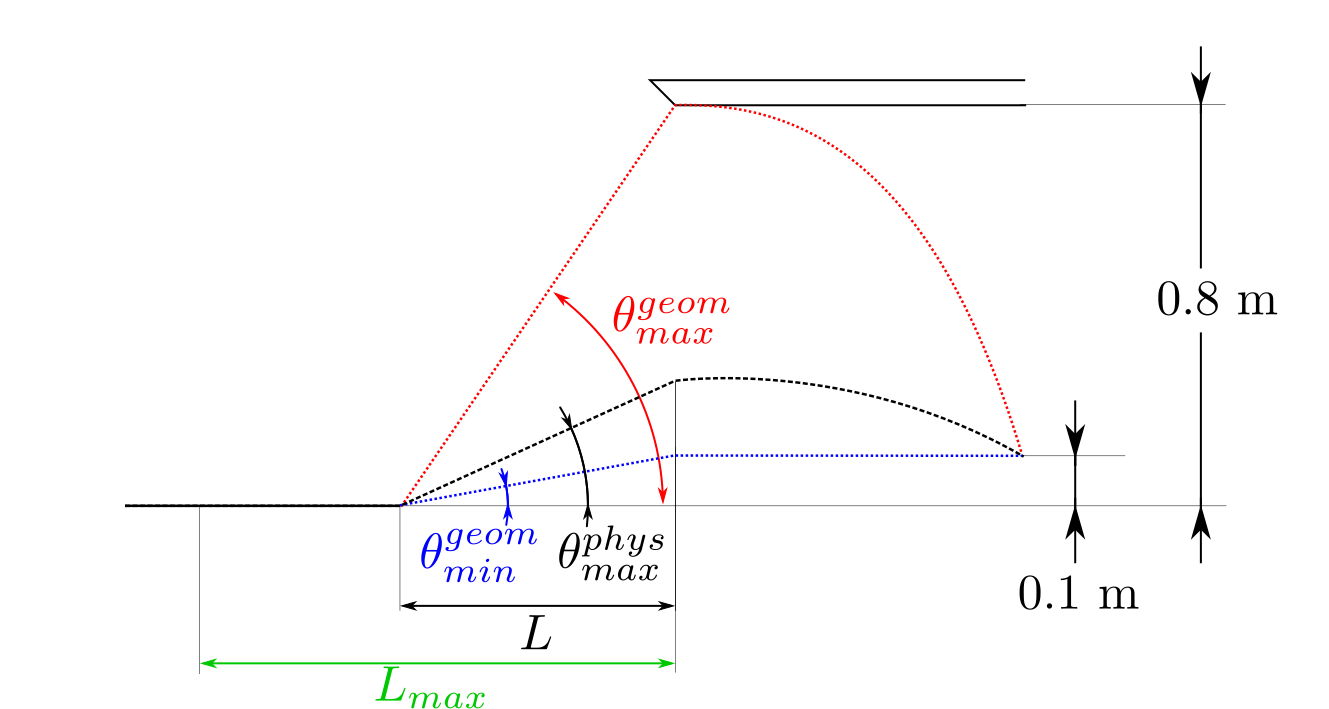
\includegraphics[width=0.85\textwidth]{Figures/3/diffuserConst4.png}
        \caption{Constraints for the diffuser case}
        \label{fig:diffuserConstr}
    \end{figure}

The search space is located in the grey zone (Figure \ref{fig:searchSpace}):

     \begin{figure}[h!]
        \centering
        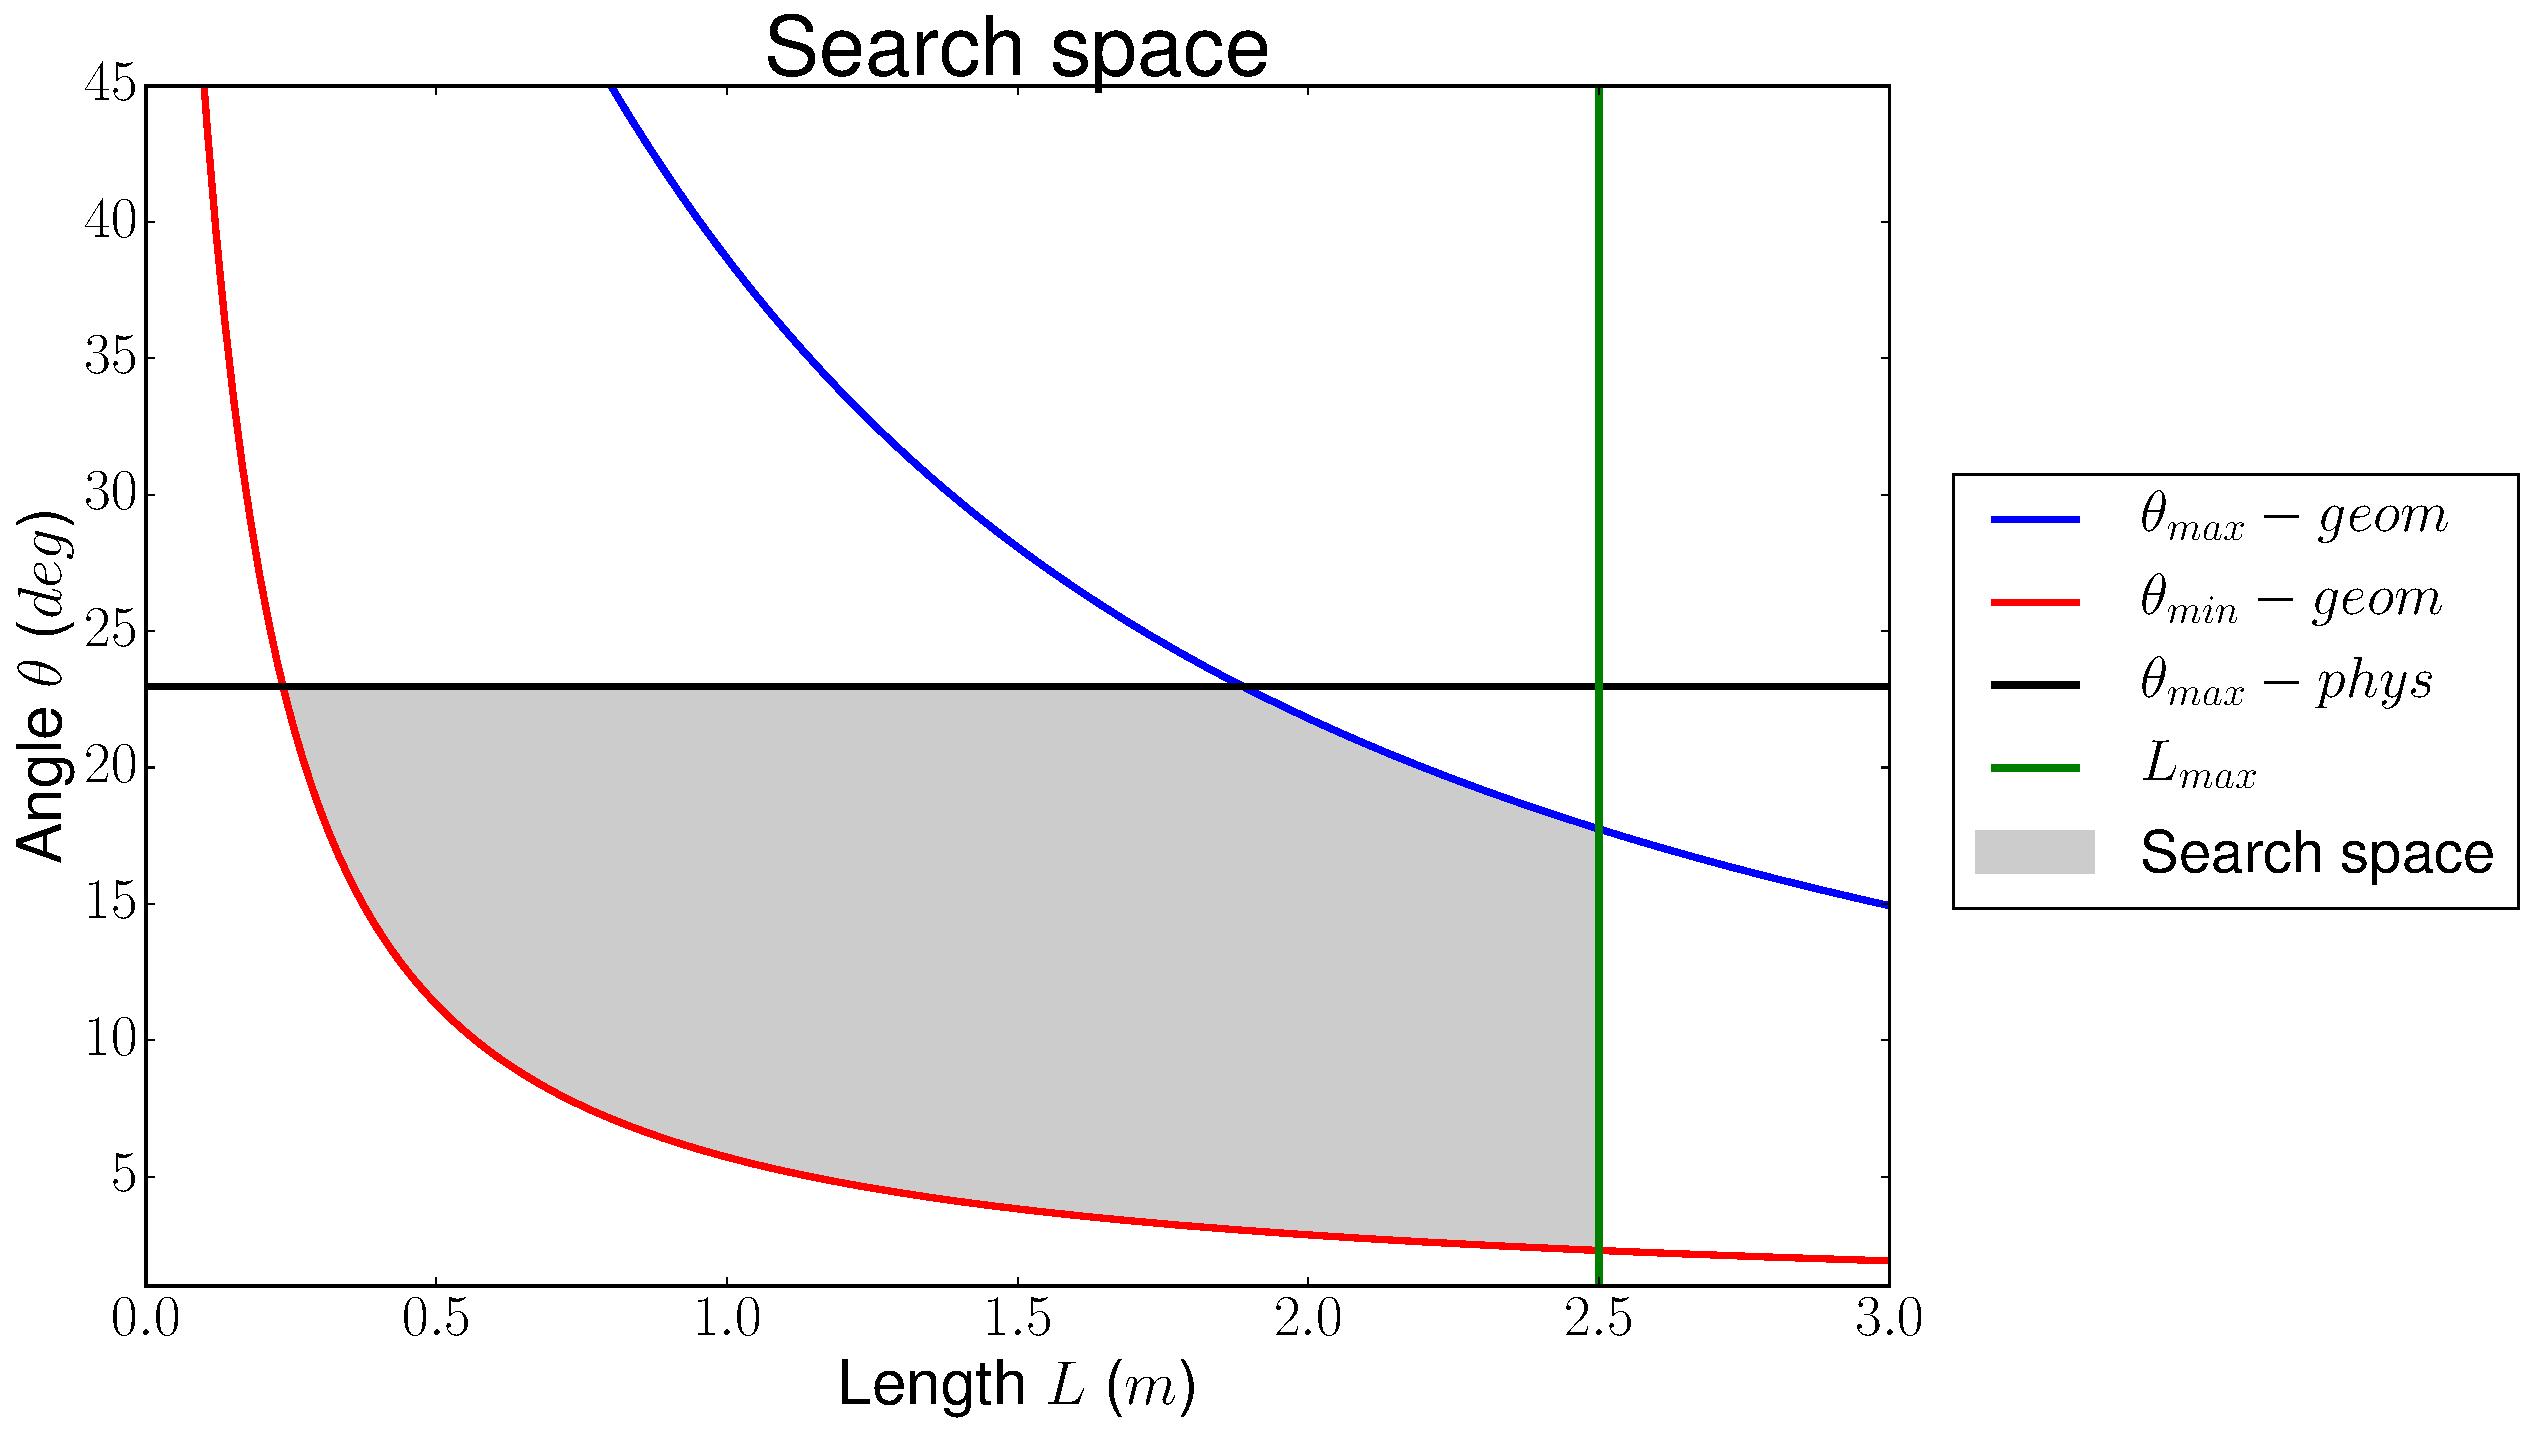
\includegraphics[width=0.85\textwidth]{Figures/3/SearchSpace.pdf}
        \caption{Search space for the diffuser analysis}
        \label{fig:searchSpace}
    \end{figure}

\newpage

The same procedure to determine the best combination of processors as the one followed in the cylinder was done for this case. Here, the optimum number of processors was 16, using a decomposition in 16 subdomains for each one of the cases. Mesh convergence was also performed, taking as most optimum values the ones obtained from a high-resolution mesh simulated with the same conditions as the case here presented. One consideration when selecting the mesh size was the time for performing each simulation, given that the simulation of one generation of 32 individuals took 2 hours, without including the fitness evaluation. 

The mesh is composed of 8 blocks with the sizes described in Figure \ref{fig:diffuserMesh}. The boundary conditions are shown in Figure \ref{fig:diffuserBC} and the type and value for each one of the variables is collected in Table \ref{table:BCdiffuser}. 

    \vspace{10mm}    
    
     \begin{figure}[h!]
        \centering
        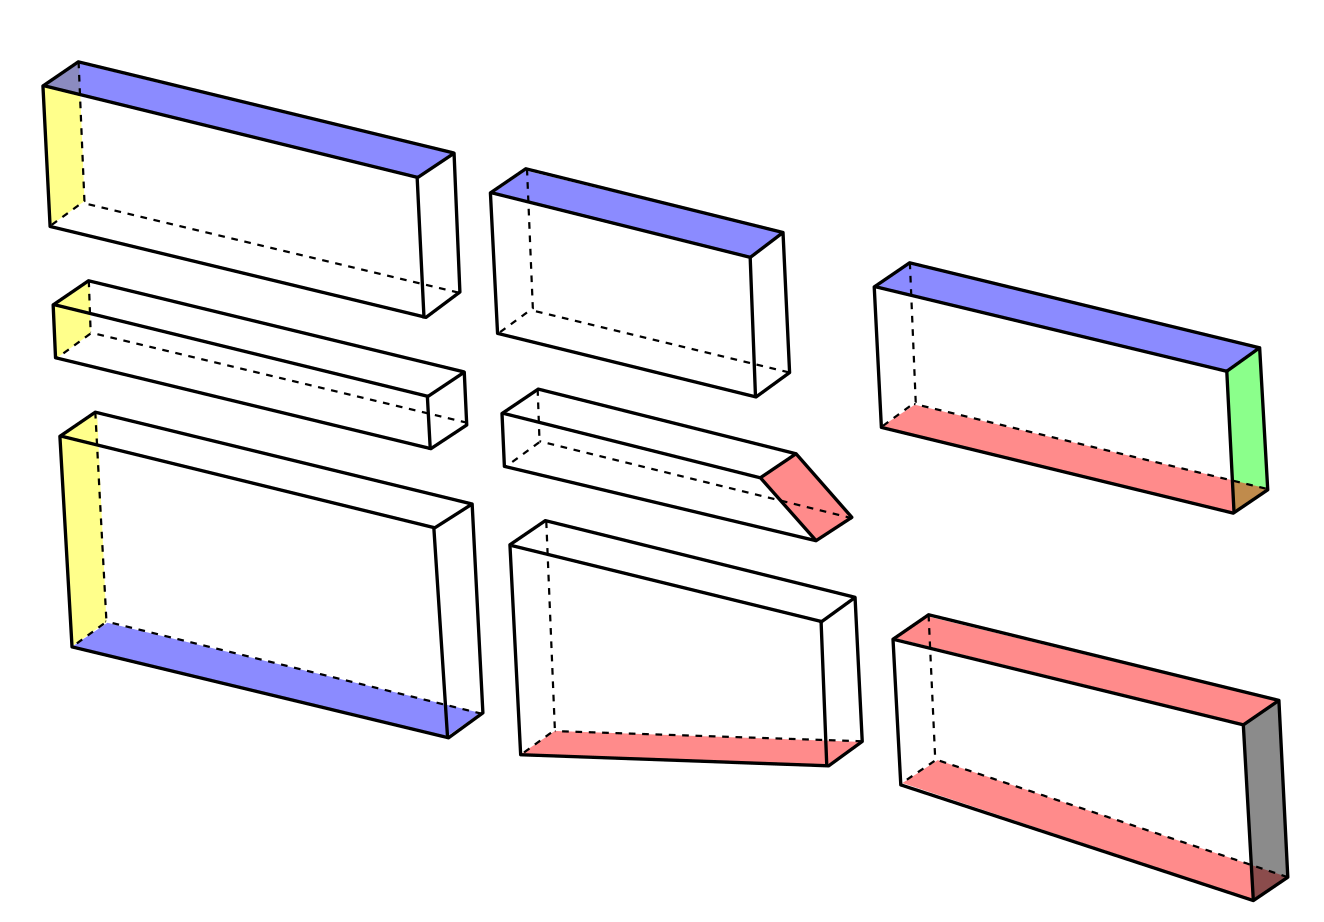
\includegraphics[width=\textwidth]{Figures/3/diffuserBC.png}
        \caption{Exploded view of the mesh for the diffuser case}
        \label{fig:diffuserBC}
    \end{figure}
    
    
\newpage
    
            \begin{table}[h!]
        \centering
           \footnotesize
        \caption{Boundary conditions for the diffuser case}
        \label{table:BCdiffuser}

        \begin{tabular}{cc}
        \multicolumn{2}{c}{\textbf{Inlet (yellow)}}          \\
        \hline
        $U$                    & \texttt{fixedValue (590 0 0)}           \\
        $p$                     &  \texttt{fixedValue 19930}          \\
        $T$                     &  \texttt{fixedValue 216}          \\
        $k$                    & \texttt{turbulentIntensityKineticEnergyInlet 2}  \\
        $\epsilon$                    &      \texttt{turbulentMixingLengthDissipationRateInlet 200} \\
        $\nu_t$                    & \texttt{calculated 0.00001}           \\
        $\alpha_t$                    & \texttt{calculated 0.01}           \\
        & \\
        \multicolumn{2}{c}{\textbf{Outlet (green)}}          \\
        \hline
        $U$                   & \texttt{zeroGradient}           \\
        $p$                     &  \texttt{zeroGradient}          \\
        $T$                     &  \texttt{zeroGradient}          \\
        $k$                    & \texttt{inletOutlet 2}           \\
        $\epsilon$                    & \texttt{inletOutlet 200}           \\
        $\nu_t$                    & \texttt{calculated 0.00001}           \\
        $\alpha_t$                    & \texttt{calculated 0.01}           \\
        & \\
        \multicolumn{2}{c}{\textbf{Engine (grey)}}      \\
        \hline
        $U$                    & \texttt{zeroGradient}           \\
        $p$                     &  \texttt{zeroGradient}          \\
        $T$                     &  \texttt{zeroGradient}          \\
        $k$                    & \texttt{inletOutlet 2}           \\
        $\epsilon$                    & \texttt{inletOutlet 200}           \\
        $\nu_t$                    & \texttt{calculated 0.00001}           \\
        $\alpha_t$                    & \texttt{calculated 0.01}           \\
        & \\
        \multicolumn{2}{c}{\textbf{Wall: cowl \& axis (red)}}           \\
        \hline
        $U$                    & \texttt{fixedValue (0 0 0)}           \\
        $p$                     &  \texttt{zeroGradient}          \\
        $T$                     &  \texttt{zeroGradient}          \\
        $k$                    & \texttt{kqRWallFunction 2}           \\
        $\epsilon$                    & \texttt{epsilonWallFunction 200}           \\
        $\nu_t$                    & \texttt{nutkWallFunction 0.0}           \\
        $\alpha_t$                    & \texttt{alphatWallFunction 0.01}           \\
        & \\

        \multicolumn{2}{c}{\textbf{Upper/Lower (blue)}}      \\
        \hline
        $U$                    & \texttt{inletOutlet (590 0 0)}           \\
        $p$                     &  \texttt{zeroGradient}          \\
        $T$                     &  \texttt{zeroGradient}          \\
        $k$                    & \texttt{inletOutlet 2}           \\
        $\epsilon$                    & \texttt{inletOutlet 200}           \\
        $\nu_t$                    & \texttt{calculated 0.00001}           \\
        $\alpha_t$                    & \texttt{calculated 0.01}           \\
                & \\

        \multicolumn{2}{c}{\textbf{Front/Back (white)}}      \\
        \hline
        $\texttt{*}$                    & empty \\
        \end{tabular}
        \end{table}

\vspace{2mm}

\newpage

\subsection{Airfoil design}


The most typical use of optimization algorithms in CFD techniques is the design of airfoils. However, the classical approach is done via adjoint shape methods, achieving the most optimum airfoil by varying the mesh shape. Other approaches try to adjust the different splines that form the airfoil applying then panel methods theory. In this study, the application of genetic algorithms and computer fluid dynamics to achieve the most optimal airfoil will be addressed. 

As said there are a lot of ways of parametrizing one airfoil. There are also families of airfoils described by some number, such as the NACA family. But for a first approach, it will be interesting to begin with a more straightforward parametrization. Joukowsky airfoils are one of those sets that are usually used for potential flow but they may be compared with some NACA airfoils, having that the transformation is more than a mathematical construction \cite{kapania2008modeling}.

Joukowsky transformation is a mathematical operation that takes one circle in the $\zeta$ complex plane and transforms it to an airfoil in the $z$ plane. The position of the circle and its radius will determine the shape of the airfoil, so the way of parametrizing the airfoil will be the $\mu_x$ and $\mu_y$ as the coordinates for the center and the radius $R$. Joukowsky transform is:
\begin{equation}
z=\zeta+\dfrac{1}{\zeta}
\end{equation}
where $z = x + y\ i$ and $\zeta = \chi + \eta\ i$. 

     \begin{figure}[h!]
        \centering
        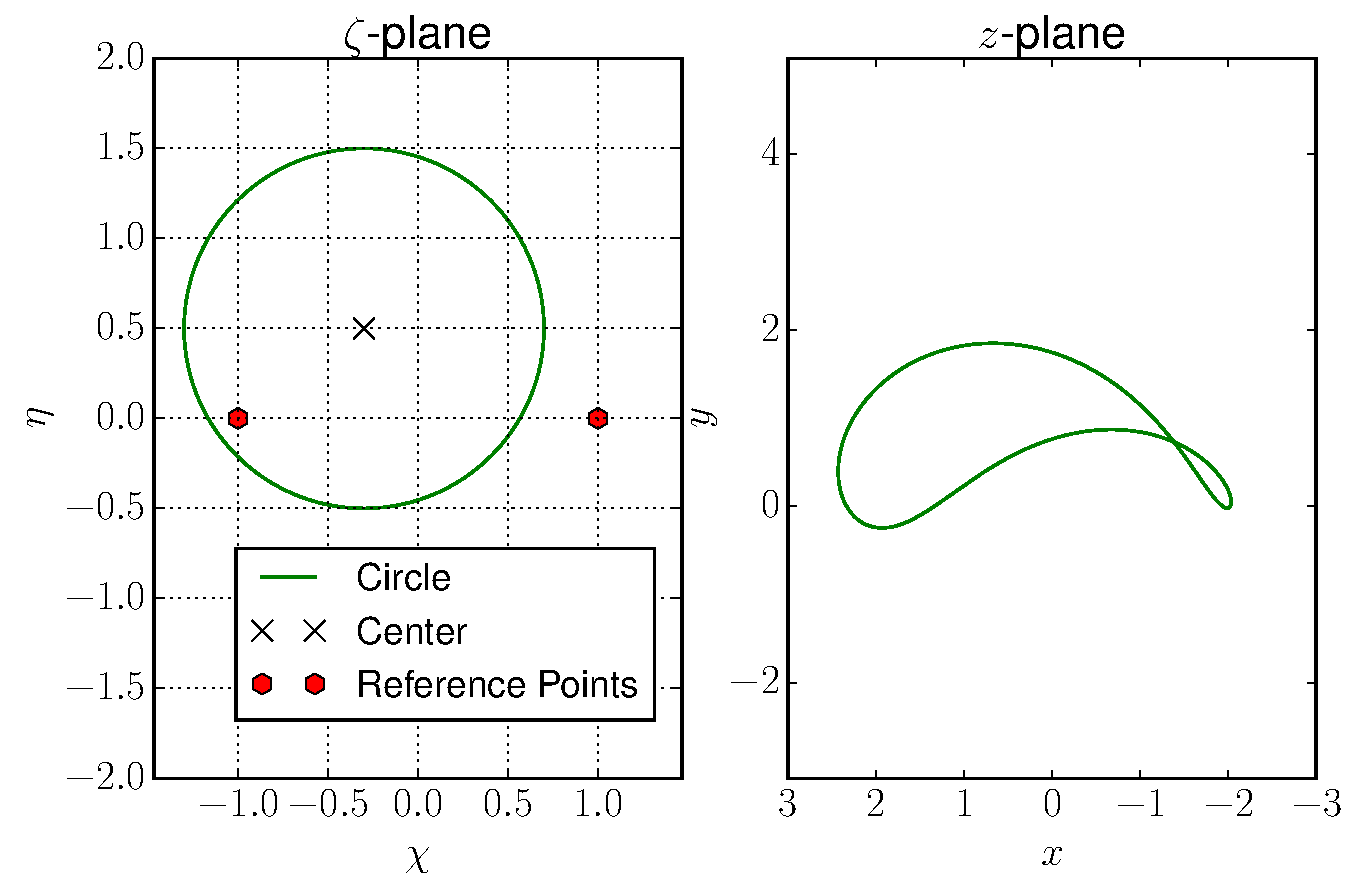
\includegraphics[width=0.8\textwidth]{Figures/3/nonJouk2.pdf}
        \caption{Example of a Joukowsky airfoil with non valid $\mu_x$, $\mu_y$ and $R$}
        \label{fig:nonJoukowsky}
    \end{figure}

\newpage

Taking a closer look to Joukowsky airfoils, they only have realistic shapes if the circle in $\zeta$ intercepts the point $\zeta = (-1,0)$ or the point $\zeta = (1,0)$ (as it can be seen in Figure \ref{fig:nonJoukowsky}). This way the radius will be determined with the position of the center of the circle, having $R=f(\mu_x,\mu_y)$. Thus the search variables that form the parameter space are $\mu_x$ and $\mu_y$, which are the coordinates of the center of the circle in the $\zeta$ plane in the $\chi$ and $\eta$.

     \begin{figure}[h!]
        \centering
        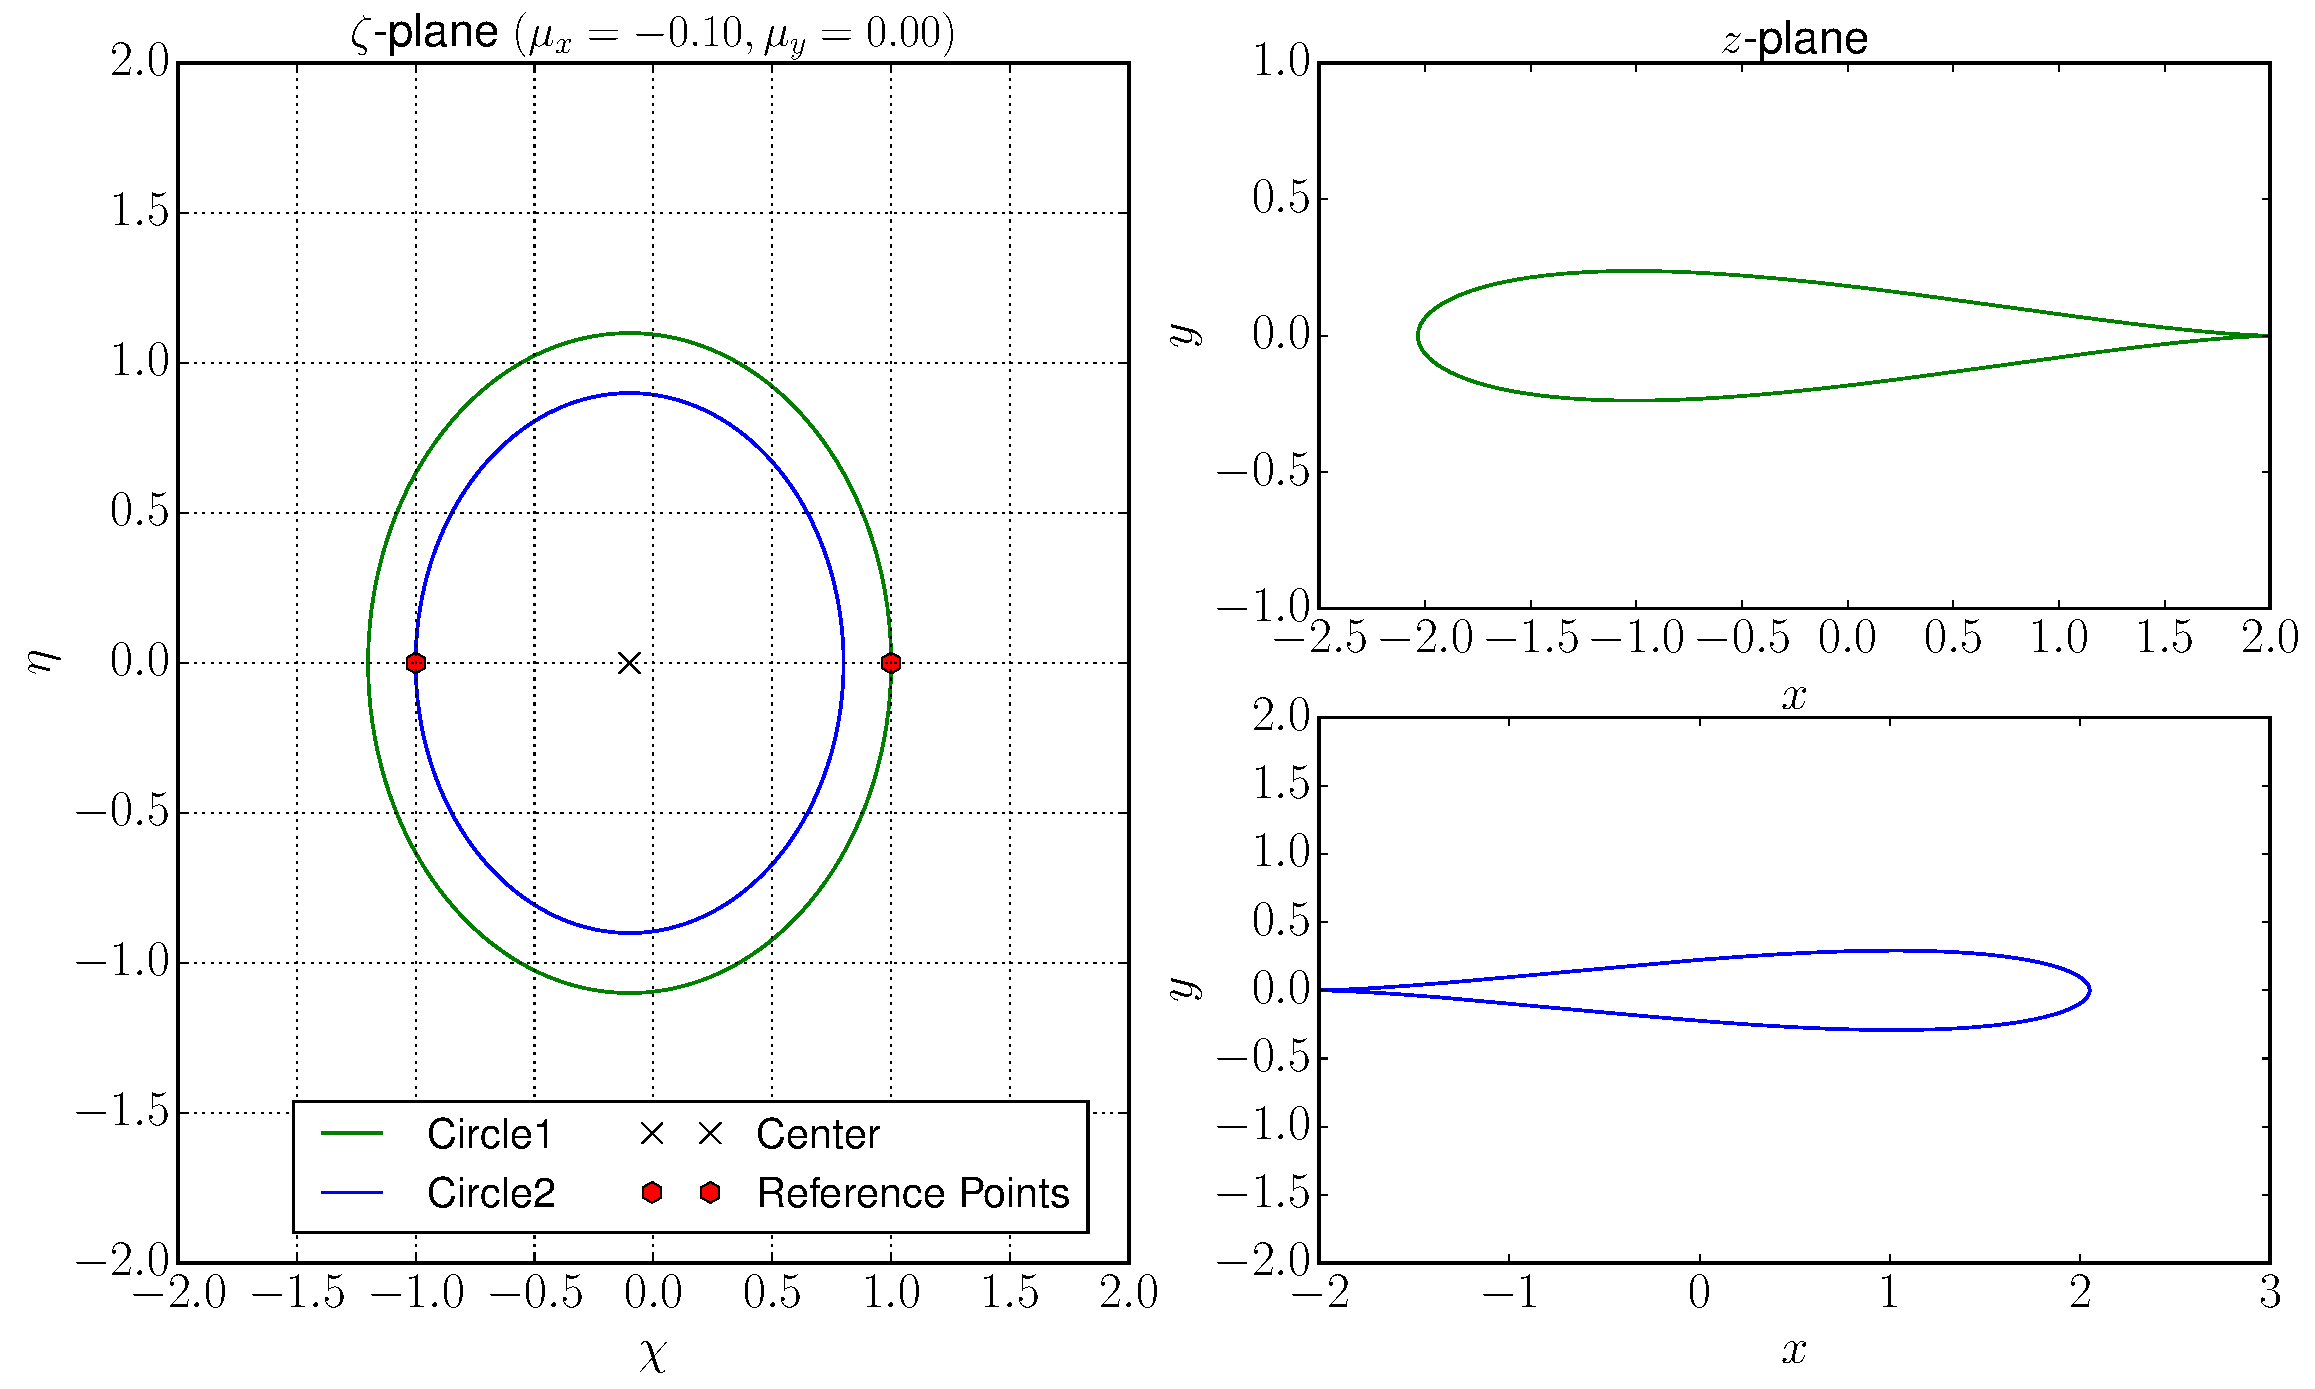
\includegraphics[width=\textwidth]{Figures/3/J_0.pdf}
        \caption{Example of a Joukowsky airfoil defined just with $\mu_x$ and $\mu_y$}
        \label{fig:joukowskyTheory}
    \end{figure}
    
Two simulations were carried out, selecting different objectives to define the function space. These objectives can be easily changed by simply varying the \texttt{fitness.py} script, where the objectives are selected and saved to create the next generation:

\begin{itemize}
    \item Maximization of lift and minimization of drag: these are the most common objectives when trying to optimize an airfoil. Nevertheless, it is impossible to get the optimum value of both at the same time.
    \item Maximization of lift-to-drag ratio and maximization of the airfoil area: this kind of objectives also try to maximize lift and minimize drag (mixed in the $L/D$ ratio) while keeping the inner area of the airfoil as bigger as possible (provided that airfoils carry the fuel in the wings it will be interesting to maximize it). 
\end{itemize}

\newpage

\subsubsection*{Case setup}

In this case, the individuals will have the search space variables represented in the mesh. The shape of the airfoil will depend on the value of $\mu_x$ and $\mu_y$, which are the search variables. The search space will be bounded inside the range $\mu_x\in[-0.3,-0.1]$ and $\mu_y\in[0.0,0.15]$. The simulation was performed with an incompressible solver in a steady-state fashion (\texttt{simpleFoam}) for at least 2500 iterations. The turbulence was modeled with the Spalart-Allmaras RAS model and a Newtonian flow was assumed. The density was chosen at sea level ($\rho=1.225\ kg\cdot m^{-3}$) as well as the viscosity value of $\nu=1.789\times10^{-5}\ m^2\cdot s^{-1}$. The airfoil faced a free stream velocity of $30\ m\cdot s^{-1}$ with turbulence values as selected for a similar OpenFOAM tutorial case ($\tilde{\nu}=0.14$ and $\nu_t =0.14$). This corresponds to a Reynolds number of $Re=2.05\times10^6$.

The mesh geometry consisted of a rectangle with a circular inlet that encased the airfoil. Joukowsky airfoils may have a wide range of possible chords, but for this analysis, the chord has been normalized to a value of one. The other dimensions of the mesh are chosen with respect to the normalized chord value and choosing them far enough so boundary conditions do not affect the flow and close enough so the computational domain is not too big. The refinement of the boundary layer was done in a very generic way, provided that the airfoil may acquire a great variety of shapes. However, and taking advantage of the fact that the mesh was done with hexahedral blocks, some boundary layer inflation was done (with simple expansion ratio gradings). 


     \begin{figure}[h!]
        \centering
        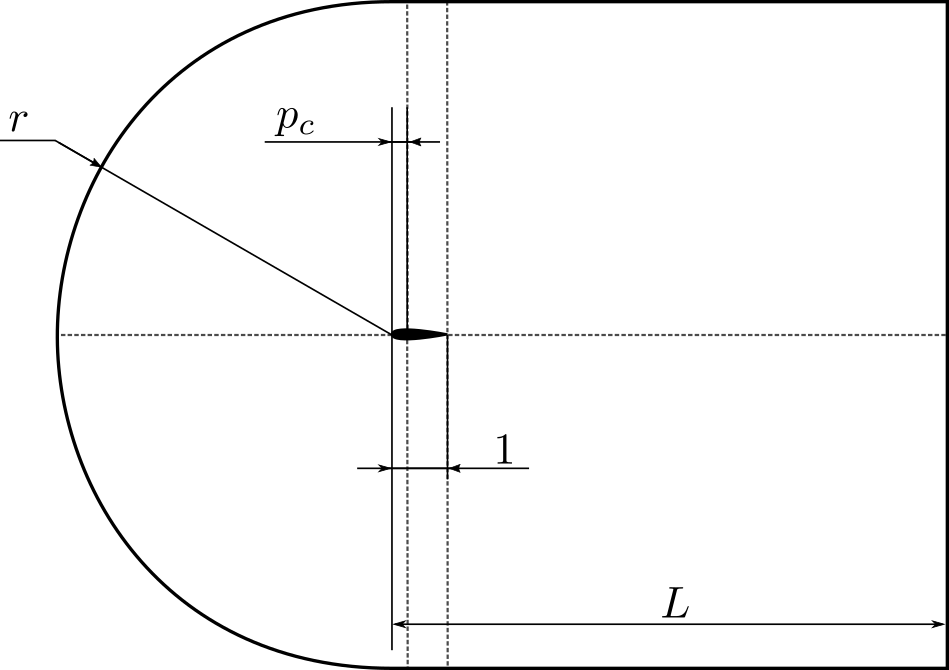
\includegraphics[width=0.7\textwidth]{Figures/3/airfoil2dReport.png}
        \caption{Mesh schematics of the airfoil}
        \label{fig:airofilMesh}
    \end{figure}

    
    
     \begin{figure}[h!]
        \centering
        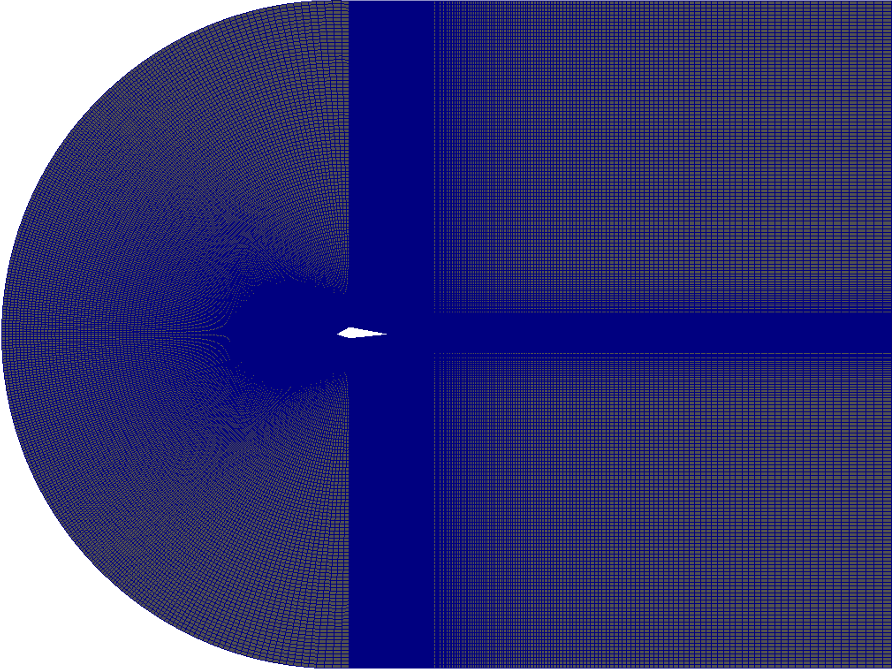
\includegraphics[width=0.7\textwidth]{Figures/3/joukOverview.png}
        \caption{Mesh for the airfoil optimization case}
        \label{fig:airofilMeshPF}
    \end{figure}

The process of creating the airfoil was automatically done with Python, but the progress of introducing the points of the spline that represents the airfoil is shown in Figures \ref{fig:uncomputedJoukowsky} and \ref{fig:computedJoukowsky}, where the airfoil is delimited by the hexahedral blocks, converting it to arcs that represent the value of $\mu_x$ and $\mu_y$.

     \begin{figure}[h!]
        \centering
        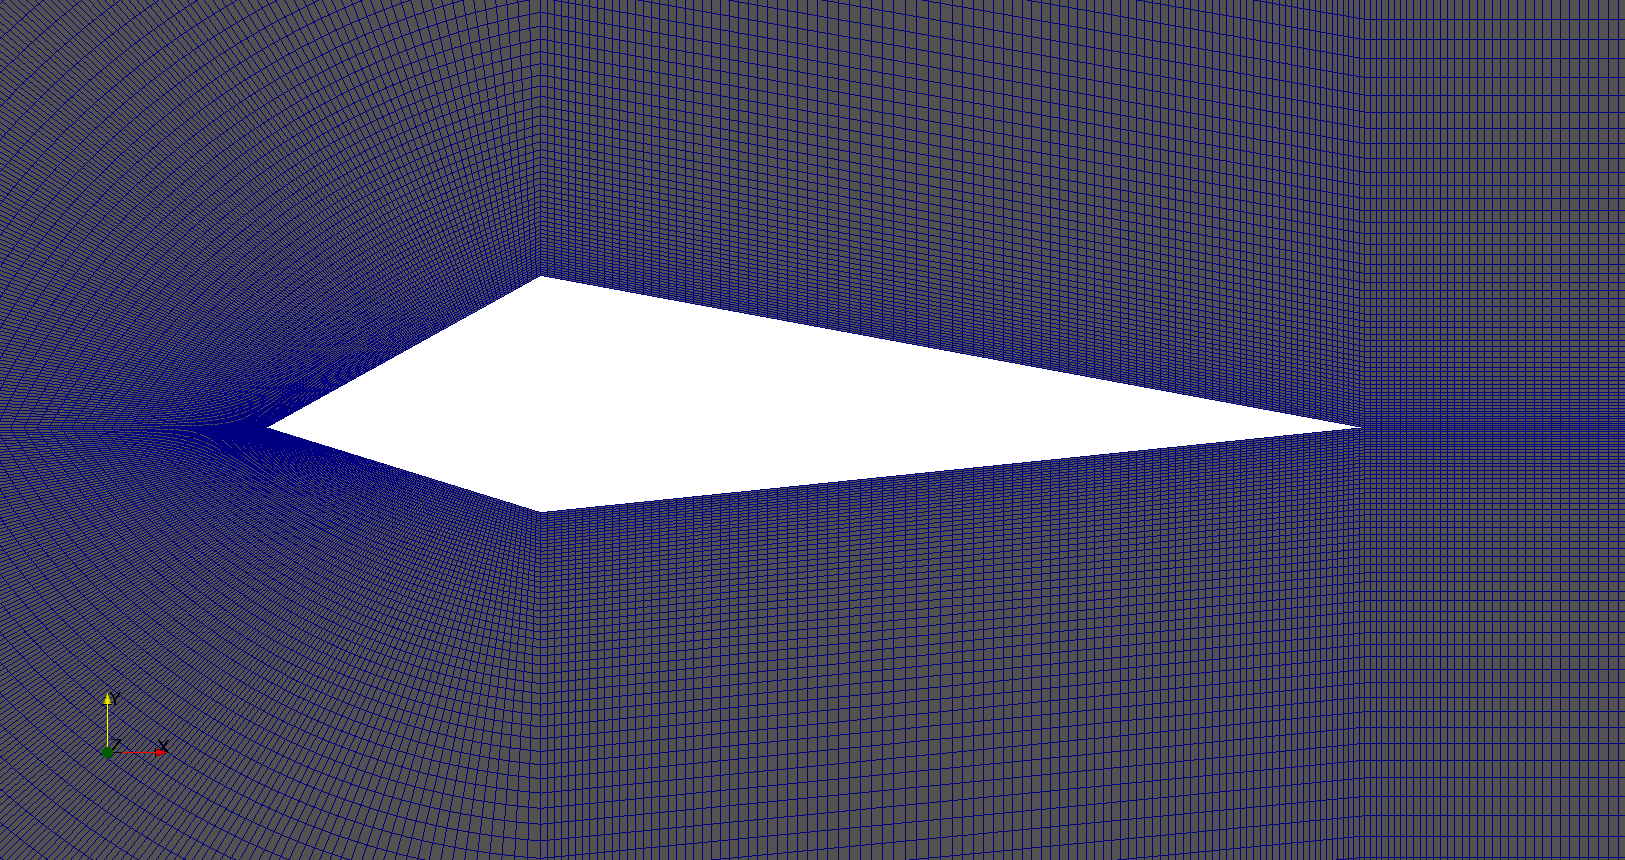
\includegraphics[width=\textwidth]{Figures/3/joukRombo.png}
        \caption{Mesh picture with the uncomputed airfoil}
        \label{fig:uncomputedJoukowsky}
    \end{figure}

    \newpage
    
     \begin{figure}[h!]
        \centering
        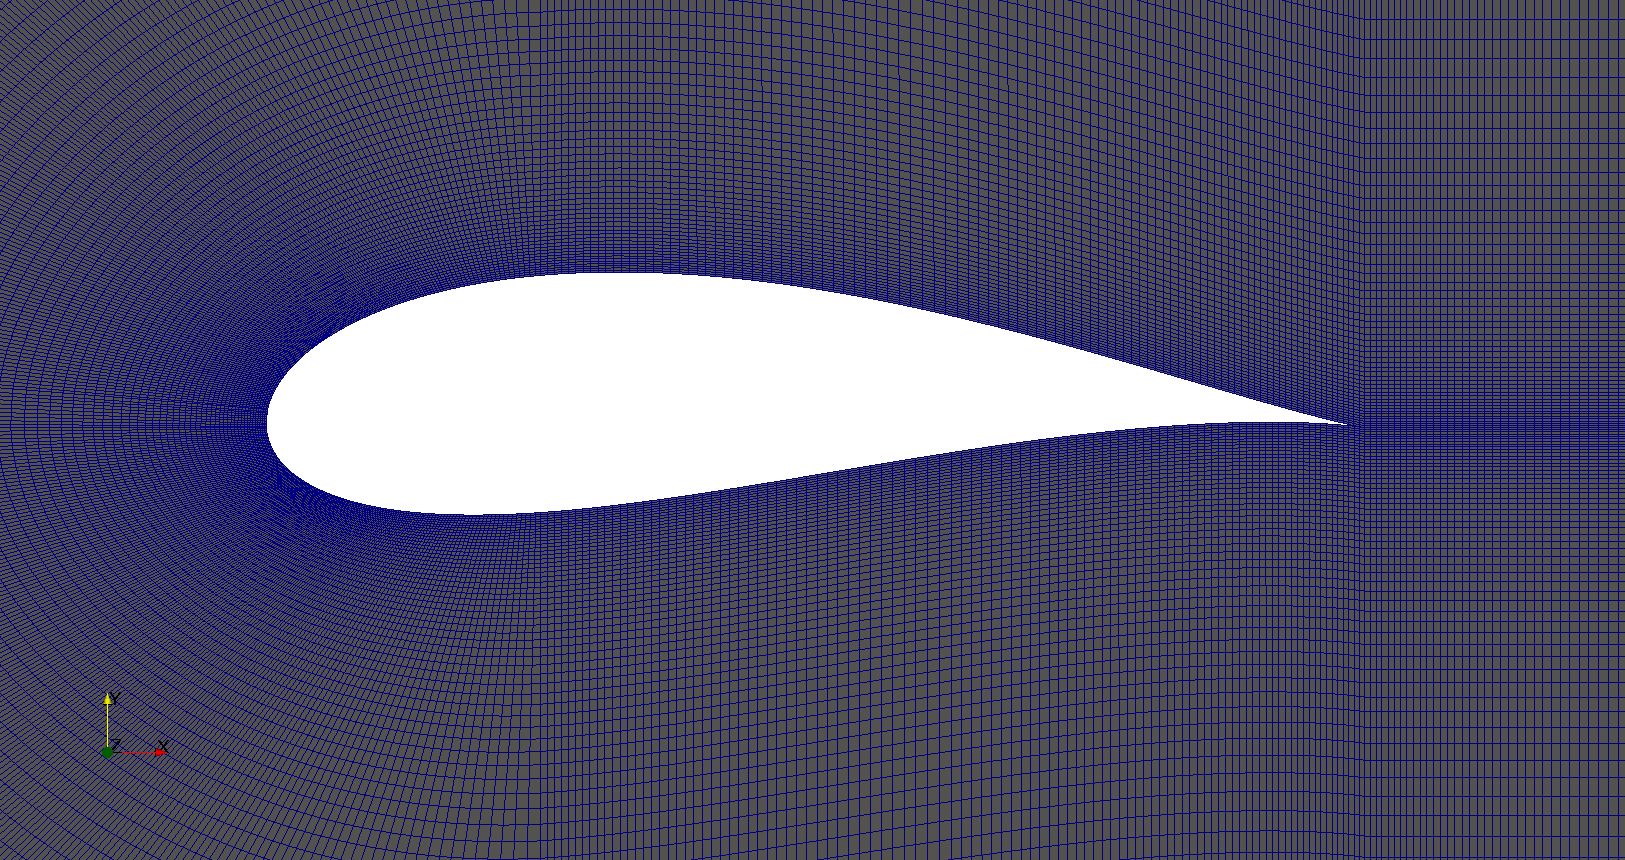
\includegraphics[width=\textwidth]{Figures/3/joukFoil.png}
        \caption{Computed airfoil in the mesh}
        \label{fig:computedJoukowsky}
    \end{figure}
        
    The boundary conditions used for the two optimization setups were the same. A freestream enters the domain through the yellow face and leaves it through the green one. Given that the angle of attack $\alpha$ is zero, there is no need of any special refinements or critical considerations about mass conservation in the domain (whereas doing angle of attack simulations will require a refined mesh and take into account the possible problems that upper and lower boundary conditions may have). 

    \vspace{3mm}    
    
     \begin{figure}[h!]
        \centering
        \small
        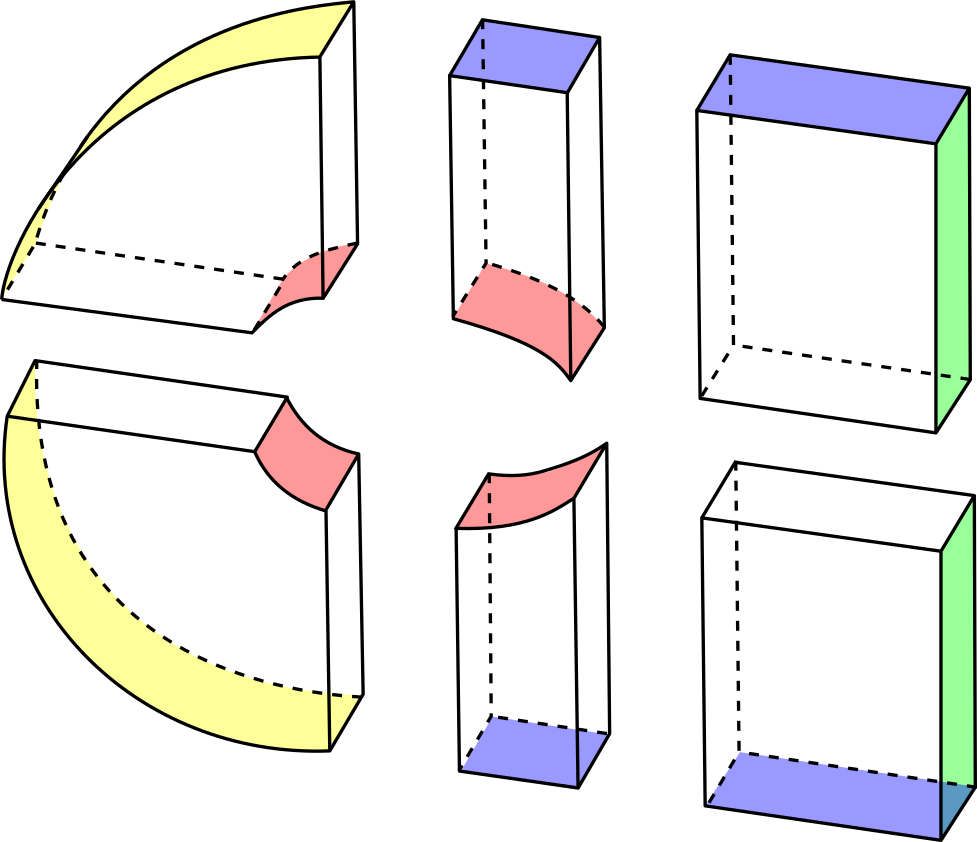
\includegraphics[width=0.5\textwidth]{Figures/3/airfoilBC.png}
        \caption{Airfoil exploded view of the mesh with the boundary conditions}
        \label{fig:airofilBCpic}
    \end{figure}
    
    \newpage
    
    The boundary conditions are listed in Table \ref{table:airfoilBC}:
   
        \begin{table}[h!]
        \centering
        \small
        \caption{Boundary conditions for the airfoil cases}
        \label{table:airfoilBC}
        \begin{tabular}{cc}
        \multicolumn{2}{c}{\textbf{Inlet (yellow)}}          \\
        \hline
        $U$                    & \texttt{freestream (30 0 0)}           \\
        $p$                     &  \texttt{freestreamPressure}          \\
        $\tilde{\nu}$                    & \texttt{freestream 0.14}           \\
        $\nu_t$                    & \texttt{freestream 0.14}           \\
                & \\

        \multicolumn{2}{c}{\textbf{Outlet (green)}}          \\
        \hline
        $U$                   & \texttt{freestream (30 0 0)}           \\
        $p$                     &  \texttt{freestreamPressure}          \\
        $\tilde{\nu}$                    & \texttt{freestream 0.14}           \\
        $\nu_t$                    & \texttt{freestream 0.14}           \\
        & \\

        \multicolumn{2}{c}{\textbf{Airfoil (red)}}           \\
        \hline
        $U$                    & \texttt{noSlip}           \\
        $p$                     &  \texttt{zeroGradient}          \\
        $\tilde{\nu}$                    & \texttt{fixedValue 0.0}           \\
        $\nu_t$                    & \texttt{nutUSpaldingWallFunction 0.0}           \\
        & \\

        \multicolumn{2}{c}{\textbf{Upper/Lower (blue)}}      \\
        \hline
        $U$                    & \texttt{freestream (30 0 0)}           \\
        $p$                     &  \texttt{freestreamPressure}          \\
        $\tilde{\nu}$                    & \texttt{freestream 0.14}           \\
        $\nu_t$                    & \texttt{freestream 0.14}           \\
                & \\
        \multicolumn{2}{c}{\textbf{Front/Back (white)}}      \\
        \hline
        $\texttt{*}$                    & empty \\
        \end{tabular}
        \end{table}